\documentclass[10pt, a4paper]{article}
\usepackage[utf8]{inputenc}
\usepackage[paper=a4paper, left=1.5cm, right=1.5cm, bottom=1.5cm, top=3.5cm]{geometry}
\usepackage[spanish]{babel}
\usepackage{indentfirst}
\usepackage{fancyhdr}
\usepackage{latexsym}
\usepackage{lastpage}
\usepackage[colorlinks=true, linkcolor=blue]{hyperref}
\usepackage{calc}
\usepackage{verbatim}
\usepackage{listings}
\usepackage{amsfonts}
\usepackage{float}
\setcounter{tocdepth}{5}
\usepackage{caption}
\usepackage{subcaption}
\sloppy

\parskip=5pt % 10pt es el tamaño de fuente

% Pongo en 0 la distancia extra entre ítemes.
\let\olditemize\itemize
\def\itemize{\olditemize\itemsep=0pt}

\usepackage{caratula}

% Acomodo fancyhdr.
\pagestyle{fancy}
\thispagestyle{fancy}
\addtolength{\headheight}{1pt}
\lhead{S. Aboy Solanes, E. Almansi, F. Canay, F. Decroix}
\rhead{$2^{\mathrm{do}}$ cuatrimestre de 2014}
\cfoot{\thepage /\pageref{LastPage}}
\rfoot{Trabajo Práctico 1 - Wiretapping}
\renewcommand{\footrulewidth}{0.4pt}

\begin{document}


\titulo{Trabajo Práctico 1 - Wiretapping}
\fecha{Martes 23 de Septiembre}
\materia{Teoría de las Comunicaciones}
\integrante{Santiago Aboy Solanes}{175/12}{santiaboy2@hotmail.com}
\integrante{Emilio Almansi}{674/12}{ealmansi@gmail.com}
\integrante{Federico Canay}{250/12}{fcanay@hotmail.com}
\integrante{Facundo Decroix}{842/11}{fndecroix92@hotmail.com}

%Pagina de titulo e indice
\thispagestyle{empty}

\maketitle

%\thispagestyle{empty}
%\mbox{}
%\newpage
\thispagestyle{empty}
\tableofcontents

\newpage

\section{Introducción}
\label{sec:introduccion}
\section{Introducción}

En este trabajo práctico hemos desarrollado una herramienta de diagnóstico de red con el objetivo de capturar los paquetes que se envían a través de la misma, identificar los distintos protocolos utilizados y principalmente, analizar el tráfico ARP (\textit{Address Resolution Protocol}) mediante herramientas provistas por la teoría de la información. Este protocolo permite vincular identificadores de la capa de enlace (MAC) con direcciones de la capa de red (IP) de dispositivos conectados a una red local.


Hemos utilizado el lenguaje de programación Python para el desarrollo de la herramienta, valiéndonos principalmente del software de manipulación de paquetes Scapy. La captura de paquetes fue realizada sobre 4 redes que... \textbf{TODO:} Definir cuáles van a ser...



\section{Desarrollo}
\label{sec:desarrollo}
\subsection{Modelos de fuente de información}
\label{subsec:modelos-fuente-informacion}

Para analizar las redes locales estudiadas, utilizamos dos modelos de fuente de información:
\vspace*{-2mm}

\begin{itemize}
  \item $S_{dst}$ = \{$s_1$ $\cdots$ $s_n$\}, siendo $s_i$ una IP que aparece como dirección destino en los paquetes ARP \emph{who-has}.
  \item $S_{src}$ = \{$s_1$ $\cdots$ $s_n$\}, siendo $s_i$ una IP que aparece como dirección origen en los paquetes ARP \emph{who-has}.
\end{itemize}

Esto permitió, dado el flujo de paquetes de una red local, definir la \textbf{información} del evento $E_i$: ``aparición del símbolo $s_i$'' como:

$$I (E_i) = log\left(\frac{1}{P(E_i)}\right)$$

unidades de información, donde $P(E_i)$ es la probabilidad de que suceda $E_i$. Al usar $log_2$, la unidad obtenida se denomina bits.

Utilizando la definición previa se puede definir la \textbf{entropía} de una fuente ($S_{dst}$ o $S_{src}$ por ejemplo), representada por $H(S)$, como el valor medio ponderado de la cantidad de información de la aparición de cada símbolo $s_i$ que la compone.

$$H(S) = \sum_{i=1}^{n} P(E_i)\,I(E_i) = \sum_{i=1}^{n} P(E_i)\,log\left(\frac{1}{P(E_i)}\right)$$

Adicionalmente, en base a estas nociones podemos establecer un criterio para considerar que un nodo de la red se considera un \textbf{nodo distinguido} para una fuente dada: un nodo es distinguido cuando la información asociada a la aparición de su IP es menor que la entropía de dicha fuente.

\subsection{Grafo de relación entre los nodos}
\label{subsec:grafo-relacion-nodos}

Como los paquetes ARP tienen una dirección IP fuente y una dirección IP destino, surge naturalmente la siguiente relación entre IP's: IP $x$ a IP $y$ \emph{sii} se observó algún paquete ARP con dirección fuente IP $x$ y dirección destino IP $y$.

Por lo tanto, en base a una muestra de paquetes ARP de una LAN, podemos definir el grafo de relación entre los nodos en base a la relación anterior, proveyendo una noción complementaria de \textbf{nodo distinguido}, para aquellos nodos que tengan grados de entrada y/o salida muy elevados.

\section{Experimentación}
\section{Experimentación}
La experimentación consistió en capturar el tráfico de paquetes, utilizando la herramienta previamente desarrollada, en las siguientes redes: una red hogareña, un McDonalds, un Starbucks, el laboratorio del DC y en el Subte.

La herramienta desarrollada no solo captura el tráfico de paquetes, sino que también hace una distinción de tipos de paquetes (qué protocolos usan), y en caso de que sean ARP toma su IP destino. Luego, con esta información se procede a calcular las probabilidades de aparición de cada tipo de paquete, contando la cantidad de apariciones de un paquete sobre el total de los paquetes capturados. De manera análoga se calcula las probabilidades de aparición de las IPs destino en los paquetes ARP. Una vez calculadas las probabilidades, es fácil realizar el cálculo de información de cada evento y las entropías de las distintas fuentes, aplicando las fórmulas presentadas en la sección de \textit{Desarrollo}.

Luego se realizaron histogramas para tener una visualización de la cantidad de apariciones de cada evento, asi también como la información de los mismos.
Por último, realizamos un grafo que representa el tráfico de paquetes en cada red, para poder comprender con mayor claridad lo que sucede en ellas.

\newpage

\subsection{Red Hogareña}

En este experimento, capturamos los paquetes de la LAN de uno de los miembros de nuestro grupo. La medición fue realizada un día sábado desde las 12 hs hasta las 14 hs. La cantidad de paquetes capturados aproximadamente es de 125000. Sin embargo, sólo 153 de estos corresponden al protocolo ARP.

\newpage

\subsection{Red McDonald's}

Para el siguiente experimento, capturamos los paquetes de la LAN Wi-Fi pública del McDonald's ubicado en el shopping Alto Avellaneda. La medición fue realizada un día sábado desde las 18 hs hasta las 20 hs. La cantidad de paquetes capturados es de aproximadamente 65.000. De todos estos, sólo 918 corresponden al protocolo ARP.

\begin{figure}[H]
       \centering
       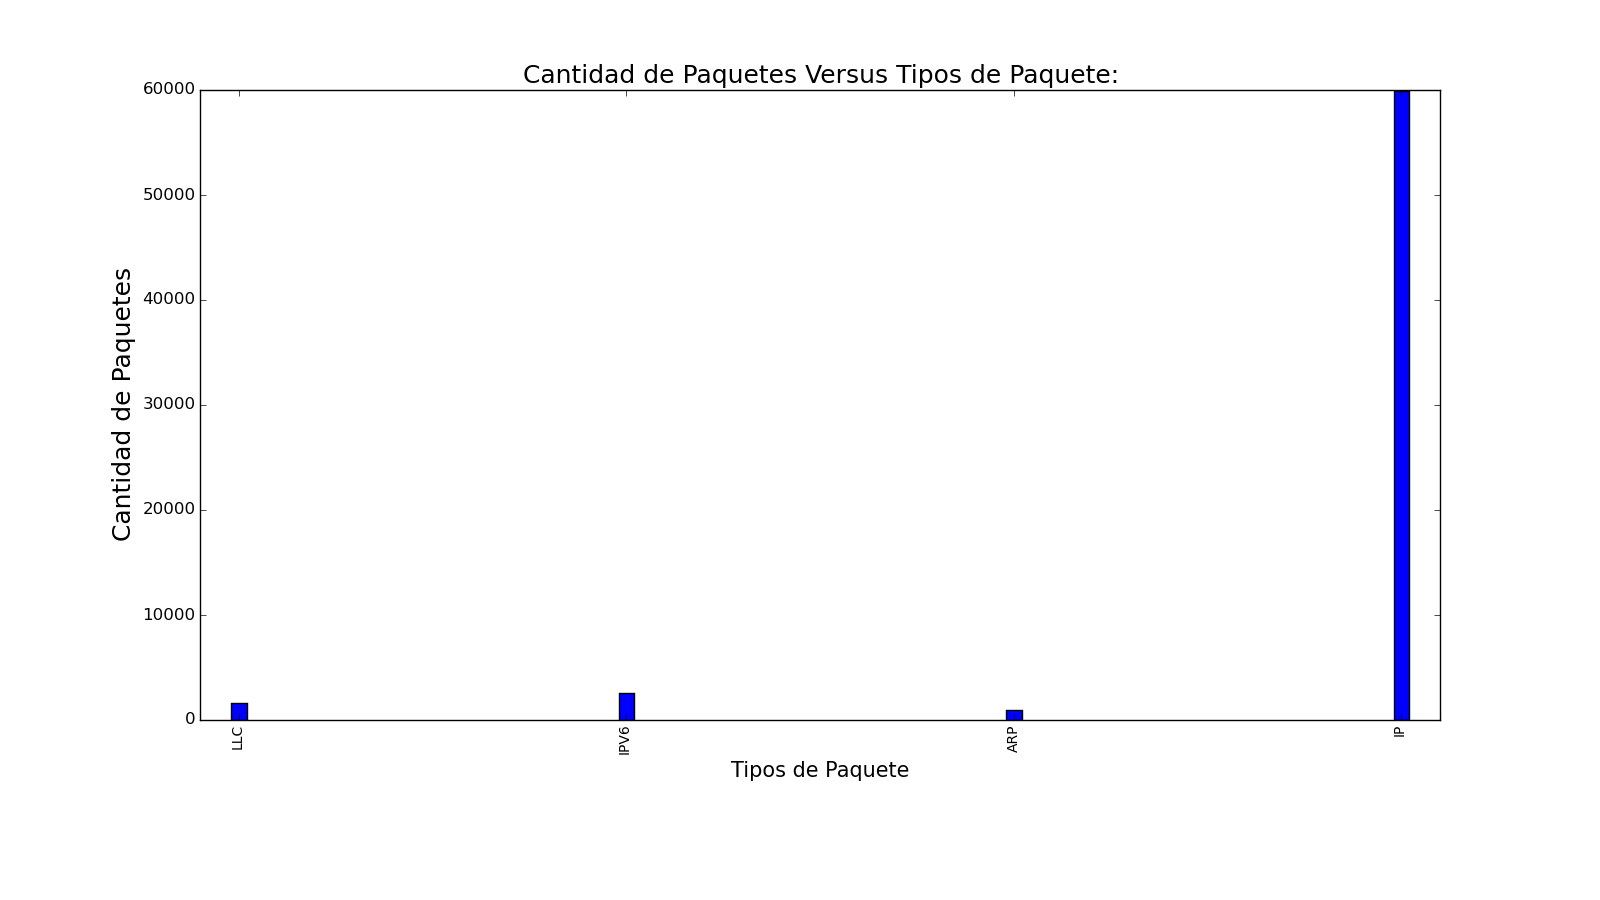
\includegraphics[width=1\textwidth]{../resultados/McDonalds/histogram_types.png}
       \caption{Protocolos de los paquetes capturados}
       \label{red-hogarena-types}
\end{figure}

\begin{figure}[H]
       \centering
       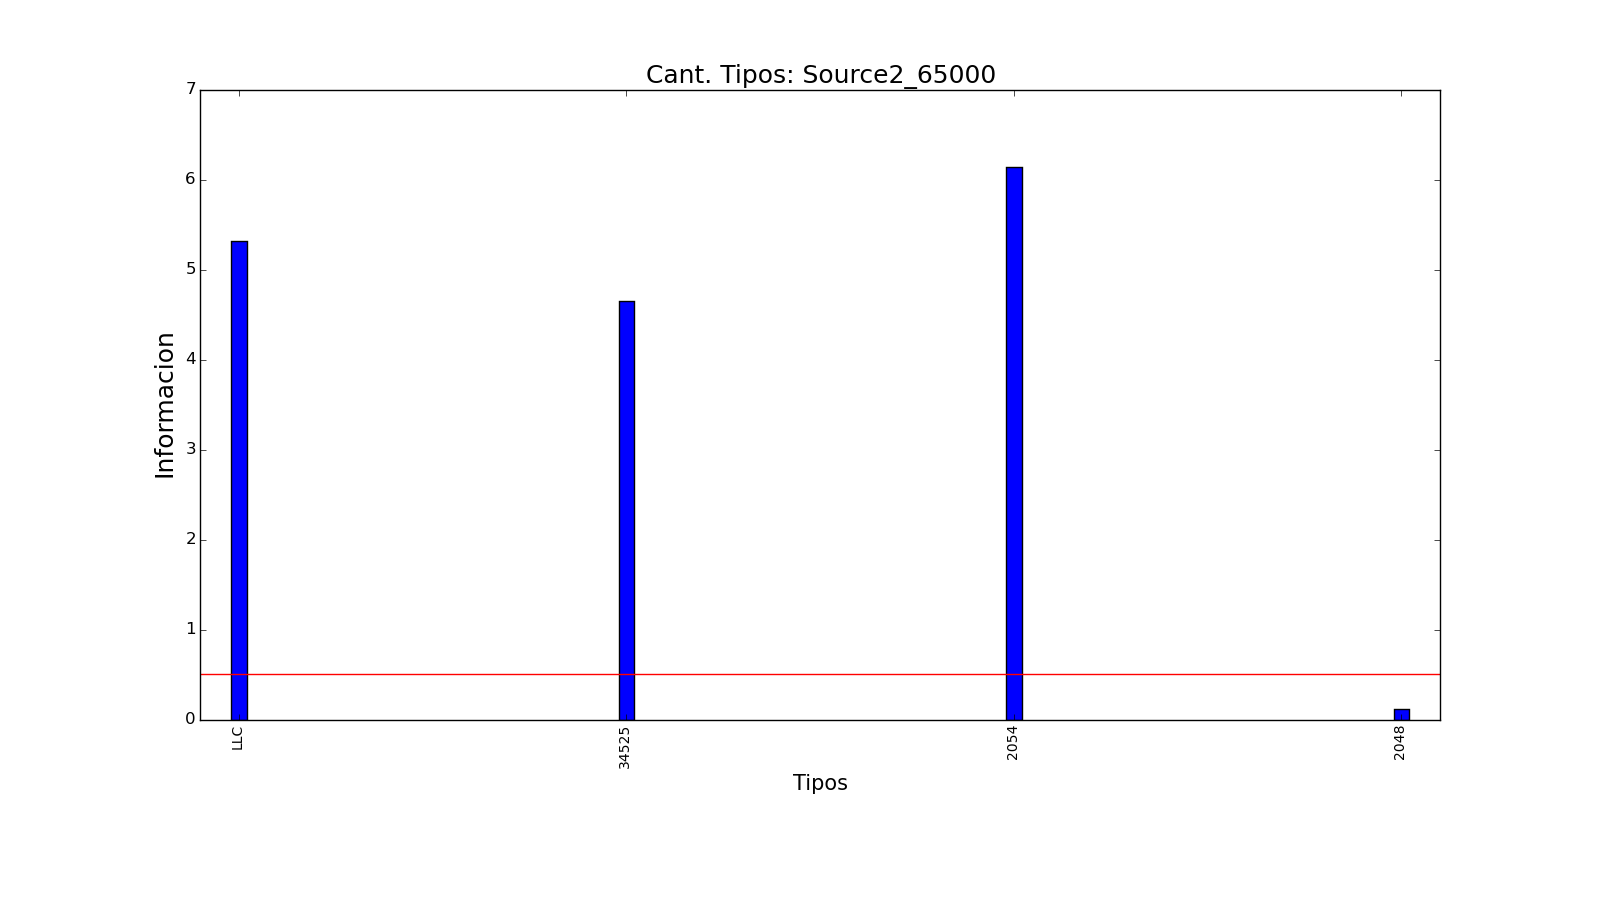
\includegraphics[width=1\textwidth]{../resultados/McDonalds/histogram_types_information.png}
       \caption{Información de los protocolos de los paquetes capturados}
       \label{red-hogarena-types}
\end{figure}


\newpage

\subsection{Red Starbucks}



\newpage

\subsection{Red Laboratorios DC}

Para este experimento, capturamos los paquetes de la LAN Wi-Fi Laboratorios-DC del Departamento de Computació de la FCEyN de la UBA. La medición fue realizada un día Lunes desde las 15hs y durante 15 minutos. La cantidad de paquetes capturados es de 4000. De estos, 164 corresponden al protocolo ARP.

\begin{figure}[H]
       \centering
       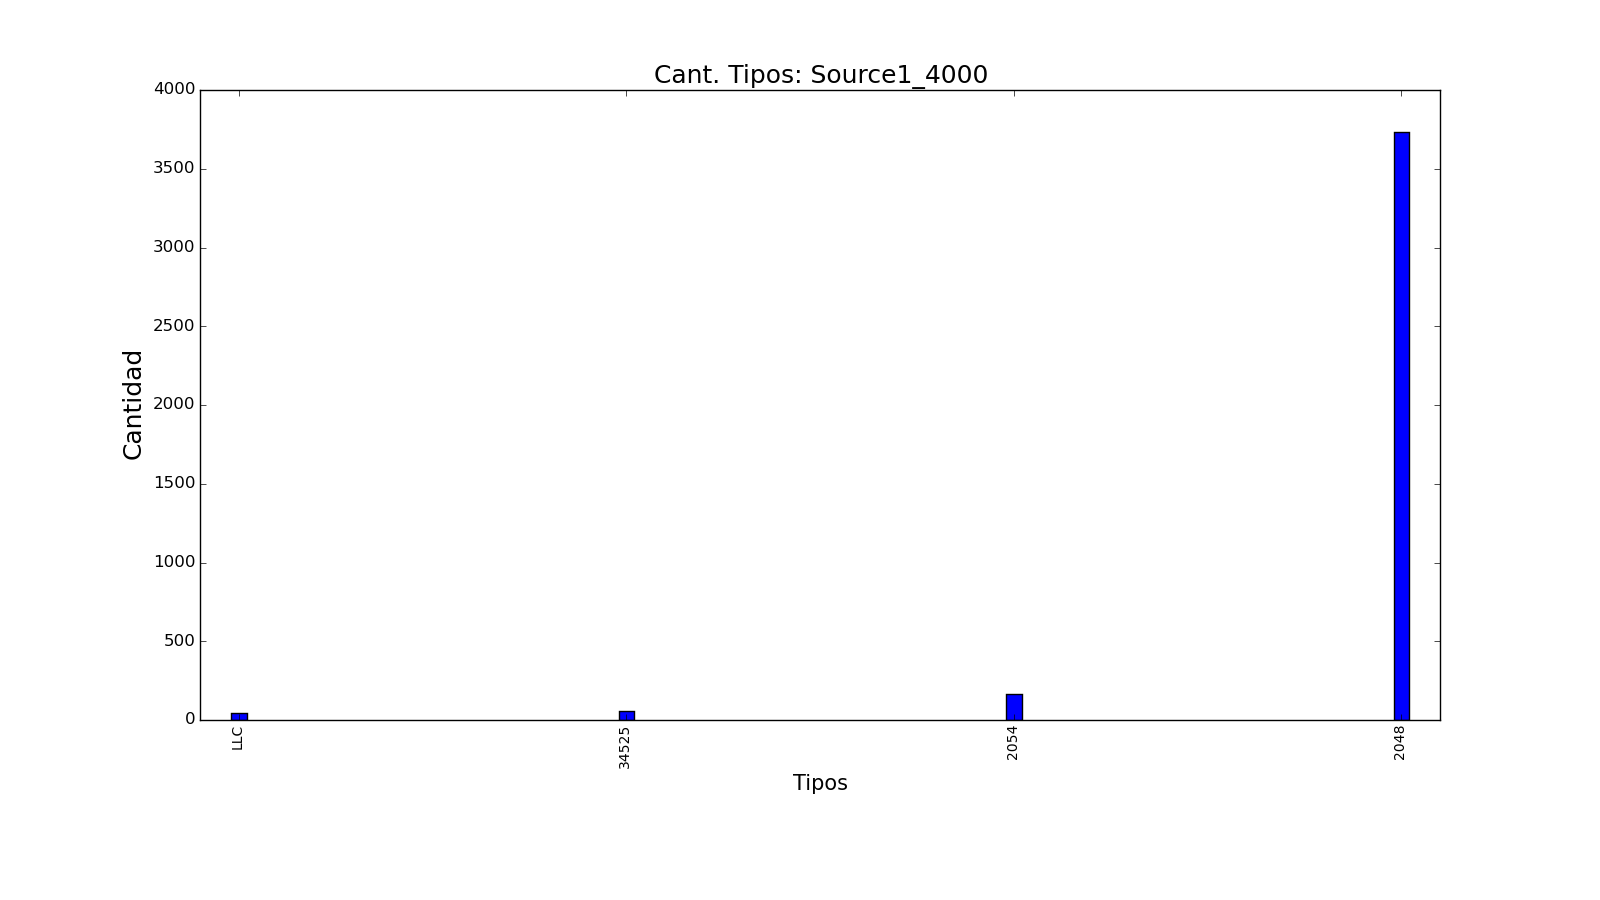
\includegraphics[width=1\textwidth]{../resultados/labo-corrida3/histogram_types.png}
       \caption{Protocolos de los paquetes capturados}
       \label{red-Starbucks-types}
\end{figure}

\begin{figure}[H]
       \centering
       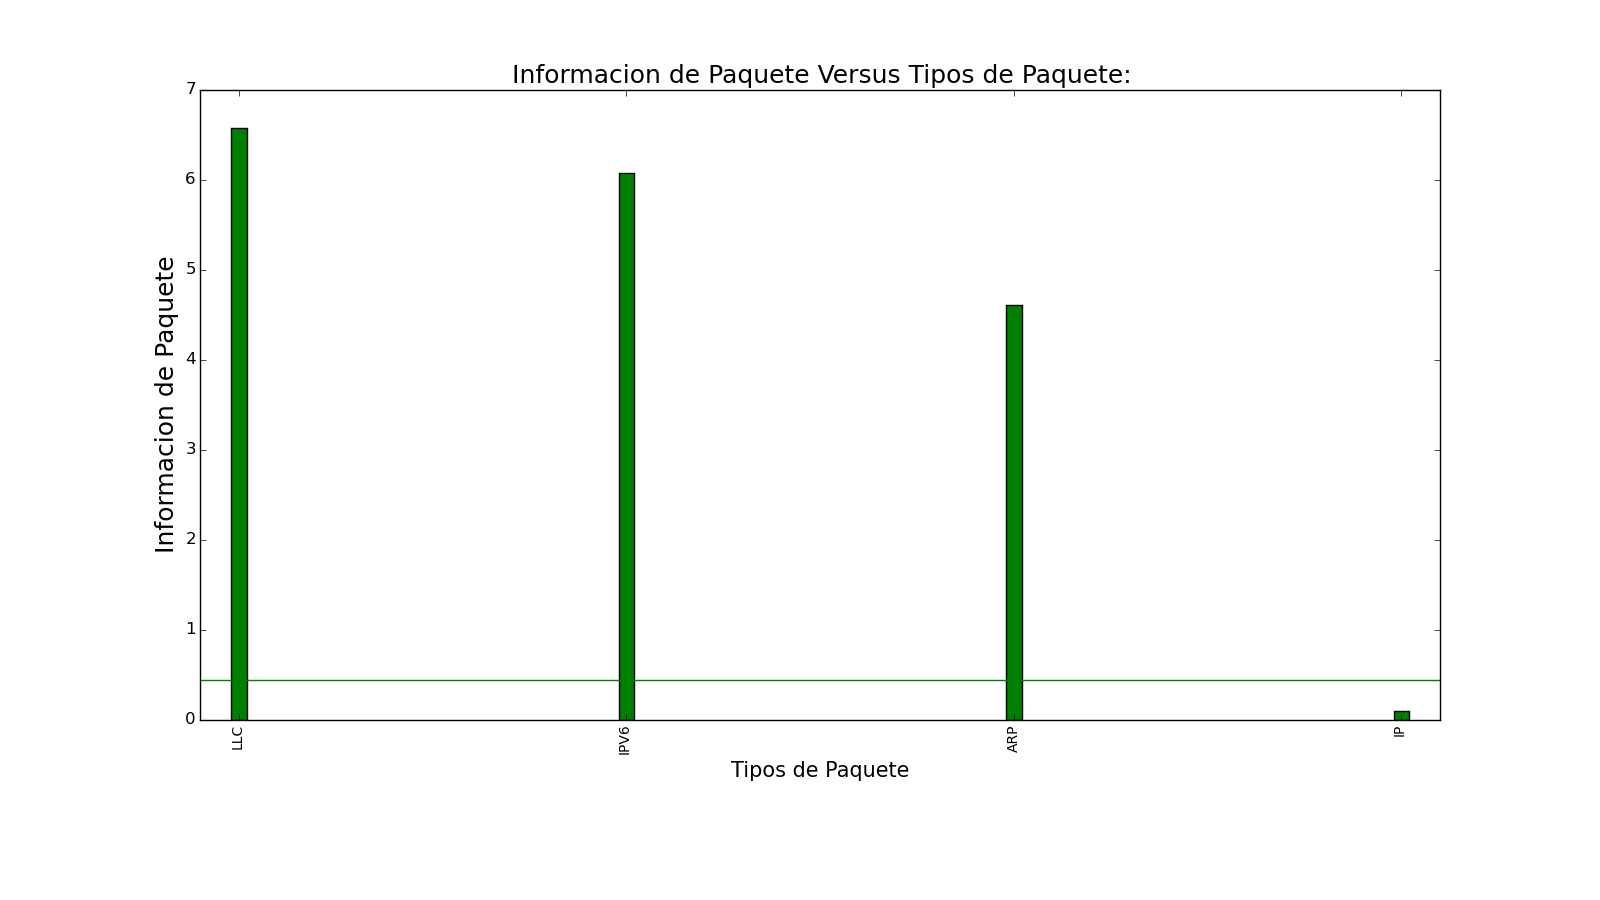
\includegraphics[width=1\textwidth]{../resultados/labo-corrida3/histogram_types_information.png}
       \caption{Información de los protocolos de los paquetes capturados}
       \label{red-Starbucks-types-information}
\end{figure}

Como podemos observar también en este experimento, de acuerdo a nuestra definición de protocolo distinguido, el protocolo IPv4 sería el único distinguido en esta fuente. Es razonable, ya que la cantidad de paquetes IPv4 es mucho mayor que la cantidad de paquetes IPv6, LLC y ARP. La información de los paquetes IPv4 es \textbf{0.0988917569855}, mientras que la entropía de la fuente es \textbf{0.440025436837}. Se observa como la información es claramente menor a la entropía.

\begin{figure}[H]
       \centering
       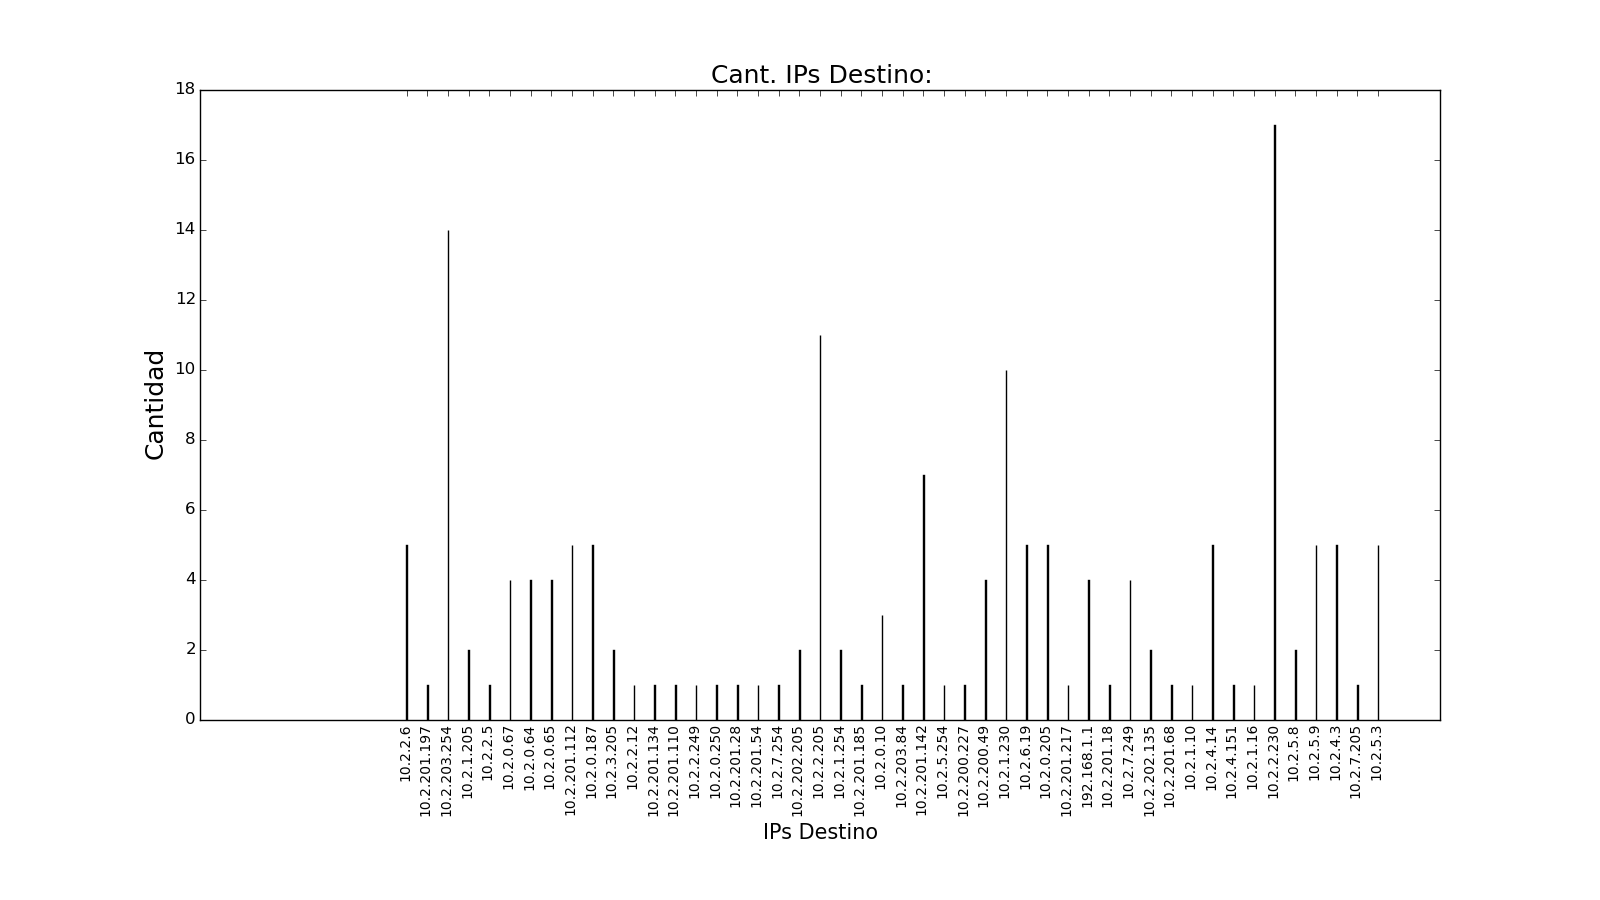
\includegraphics[width=1\textwidth]{../resultados/labo-corrida3/histogram_dst.png}
       \caption{IPs destino de los paquetes ARP}
       \label{red-Starbucks-dst}
\end{figure}

\begin{figure}[H]
       \centering
       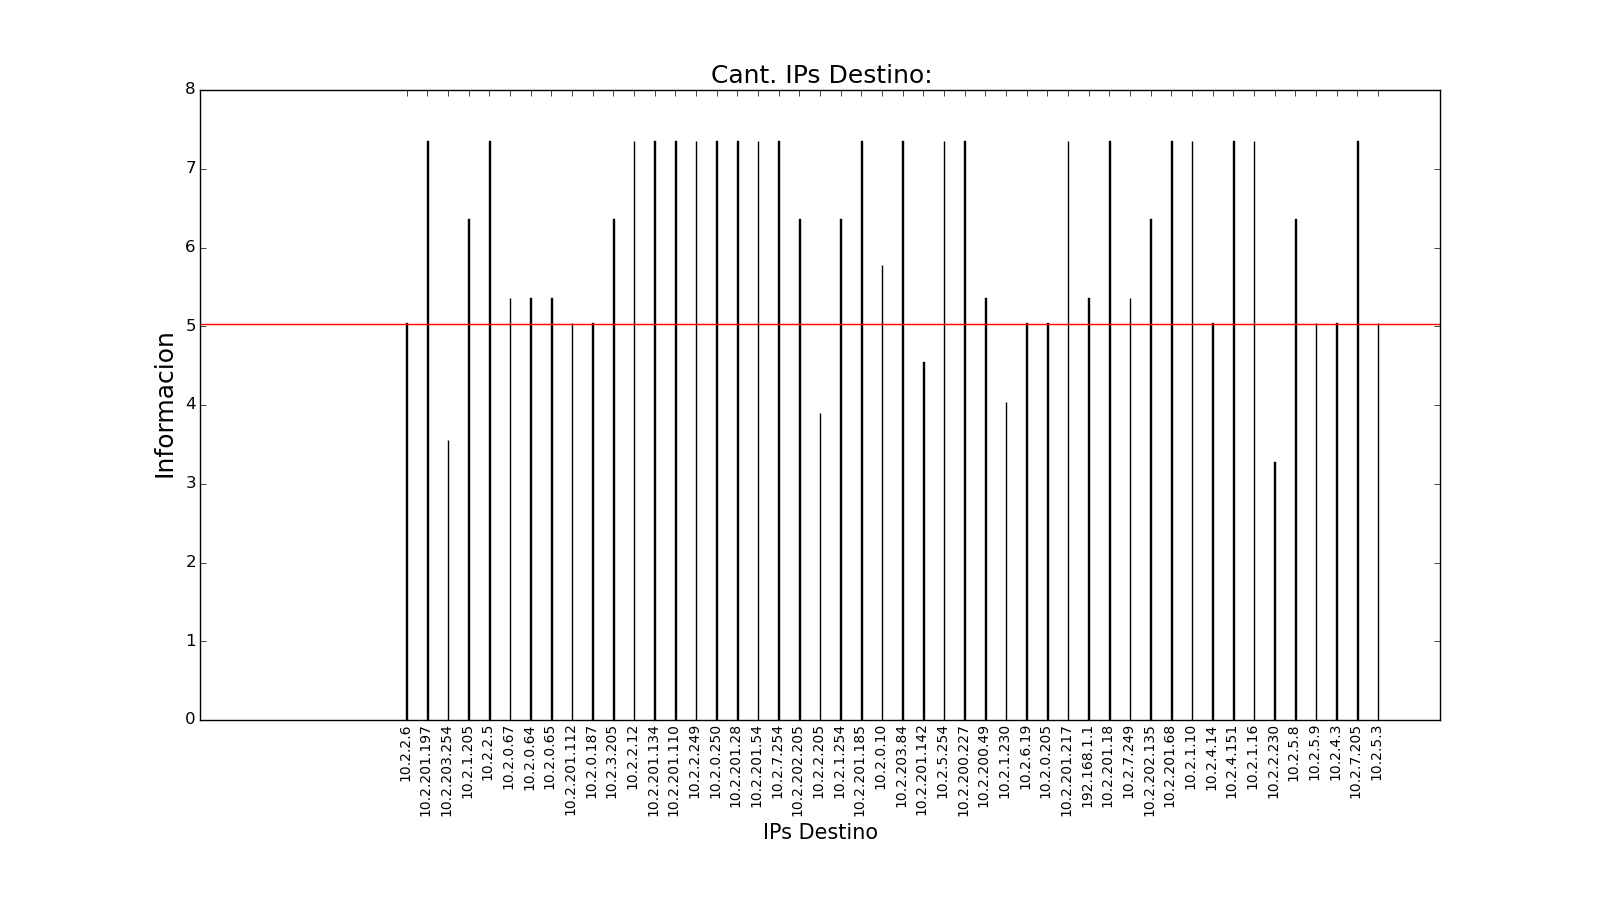
\includegraphics[width=1\textwidth]{../resultados/labo-corrida3/histogram_dst_information.png}
       \caption{Información de IPs destino de los paquetes ARP}
       \label{red-Starbucks-dst-information}
\end{figure}


\begin{figure}[H]
       \centering
       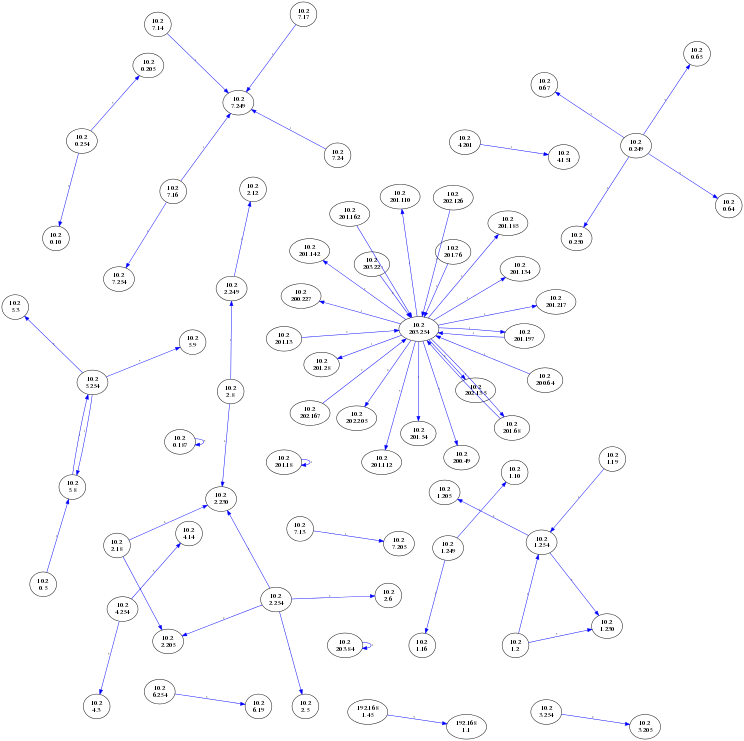
\includegraphics[width=1\textwidth]{../resultados/labo-corrida3/network.png}
       \caption{Tráfico de paquetes ARP}
       \label{red-Starbucks-dst-information}
\end{figure}

Analizando la información de estos gráficos vemos como la IP \textbf{10.2.203.254} parece ser el router: recibe una mayor cantidad de paquetes que casi todas las demás IPs, es un nodo distinguido por ser su información menor a la entropía, y las conexiones que tiene son a las IPs 10.2.200.X, 10.2.201.X y 10.2.202.X, que deben ser subnets.\\

También vemos por ejemplo que la IP \textbf{10.2.2.230} recibe incluso una mayor cantidad de paquetes y  también es un nodo distinguido, pero esa mayor cantidad de paquetes viene desde pocos nodos. Creemos por esto que puede tratarse de algún servidor (de datos, de imágenes, etcétera).

\newpage

\subsection{Red Subte D}

Para el último experimento, capturamos los paquetes de la LAN Wi-Fi Subte-BA de la estación Plaza Italia de la Línea D del Subte de Buenos Aires.La medición fue realizada un día Domingo a las 16.30hs y durante solamente 1 minuto (por motivos externos). Capturamos 1.000 paquetes de los cuales 25 son ARP.

\begin{figure}[H]
       \centering
       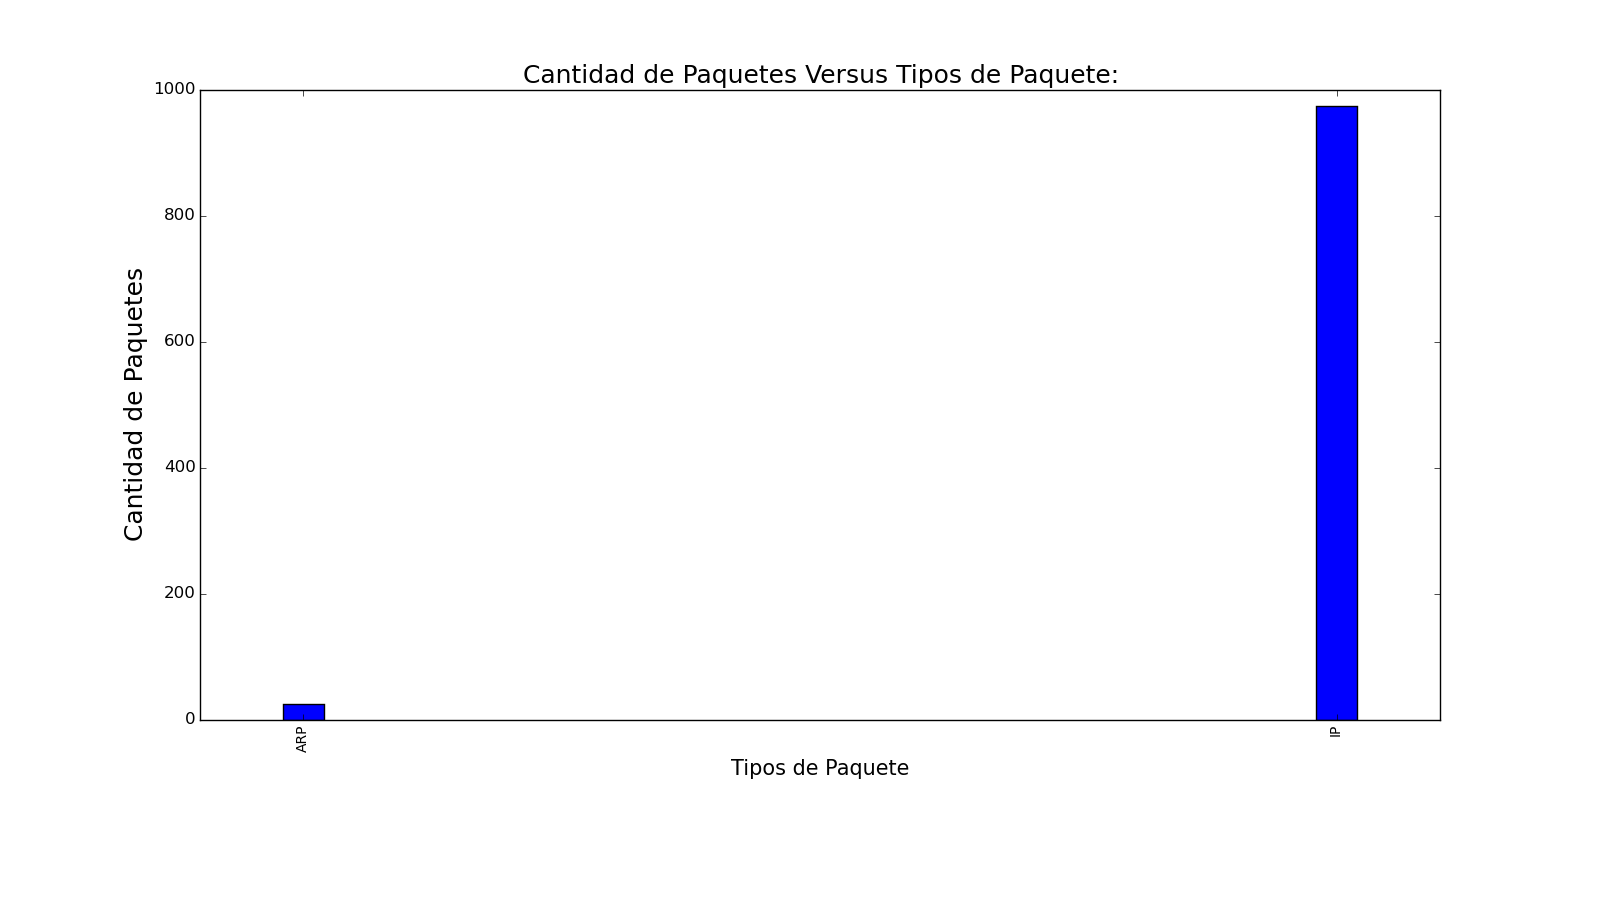
\includegraphics[width=1\textwidth]{../resultados/subte/histogram_types.png}
       \caption{Protocolos de los paquetes capturados}
       \label{red-Starbucks-types}
\end{figure}

En este caso el overhead impuesto por los paquetes ARP es de 2.5\%

\begin{figure}[H]
       \centering
       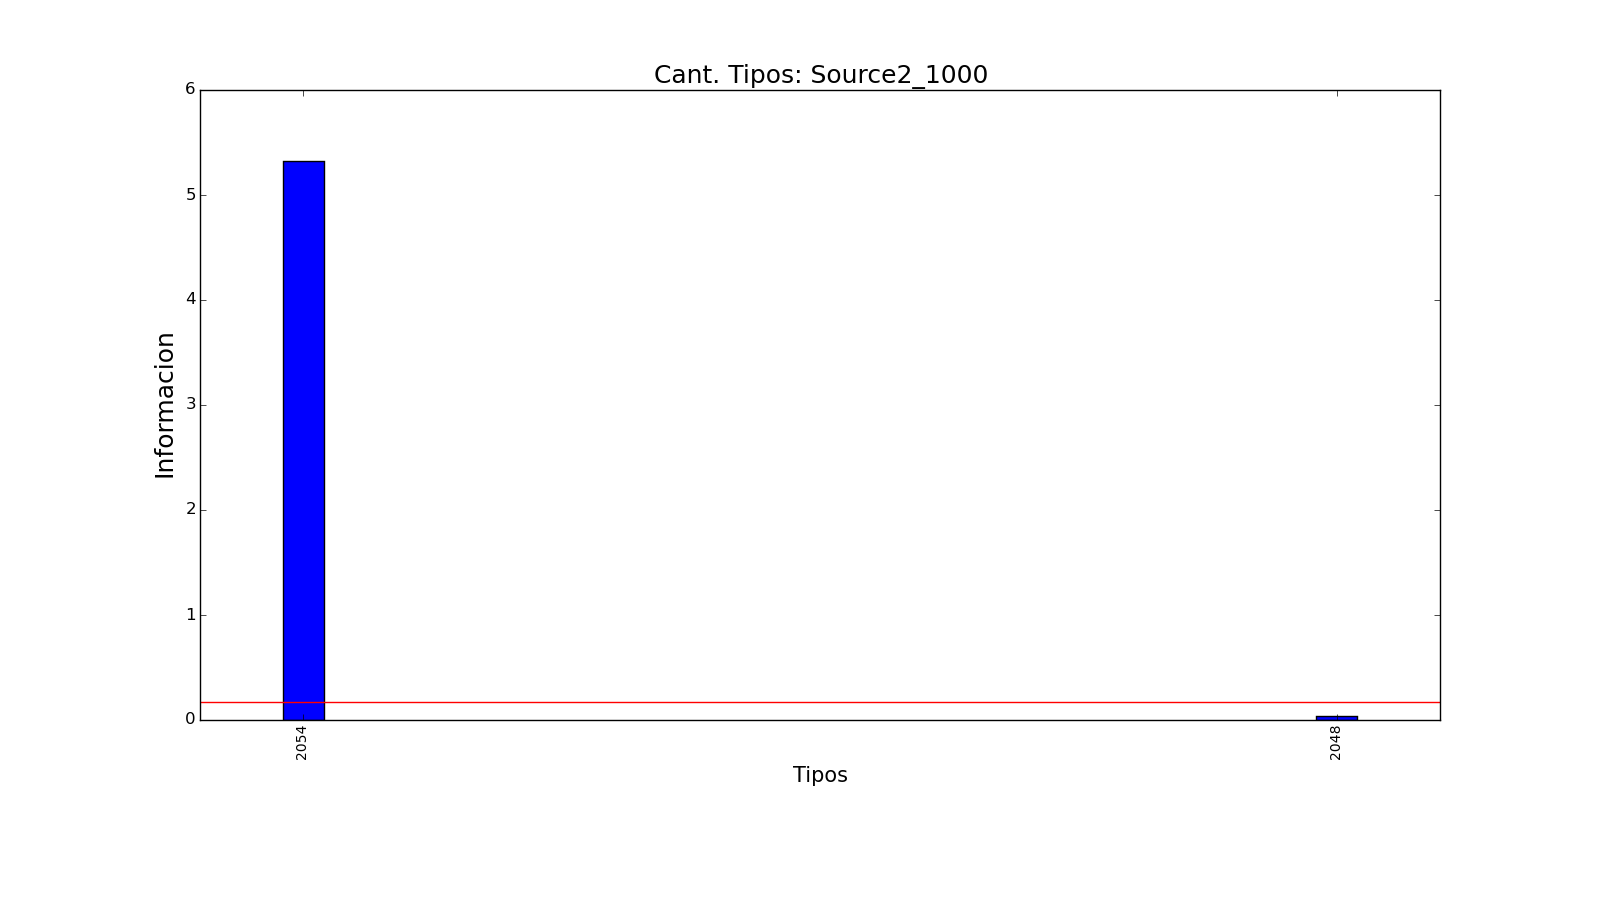
\includegraphics[width=1\textwidth]{../resultados/subte/histogram_types_information.png}
       \caption{Información de los protocolos de los paquetes capturados}
       \label{red-Starbucks-types-information}
\end{figure}

Como podemos también en este experimento, el protocolo IPv4 sería el único distinguido en esta fuente. Es razonable, ya que la cantidad de paquetes IPv4 es mucho mayor que la cantidad de paquetes ARP. La información de los paquetes IPv4 es \textbf{5.32192809489}, mientras que la entropía de la fuente es \textbf{0.168660931497}. Se observa como la información es muy menor a la entropía.

\begin{figure}[H]
       \centering
       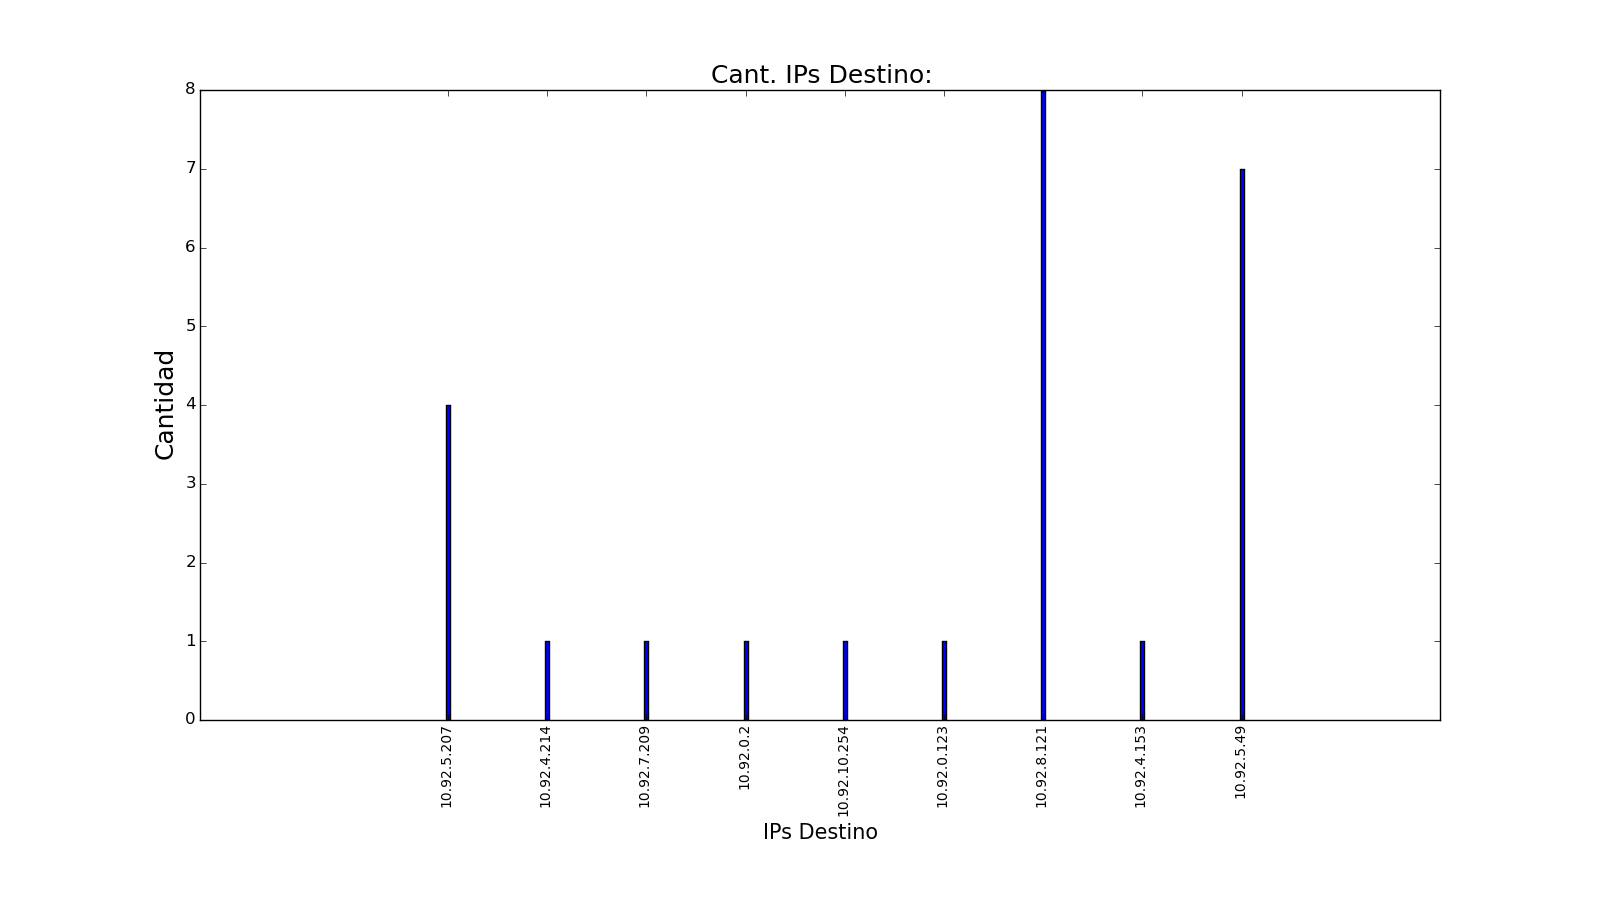
\includegraphics[width=1\textwidth]{../resultados/subte/histogram_dst.png}
       \caption{IPs destino de los paquetes ARP}
       \label{red-Starbucks-dst}
\end{figure}

\begin{figure}[H]
       \centering
       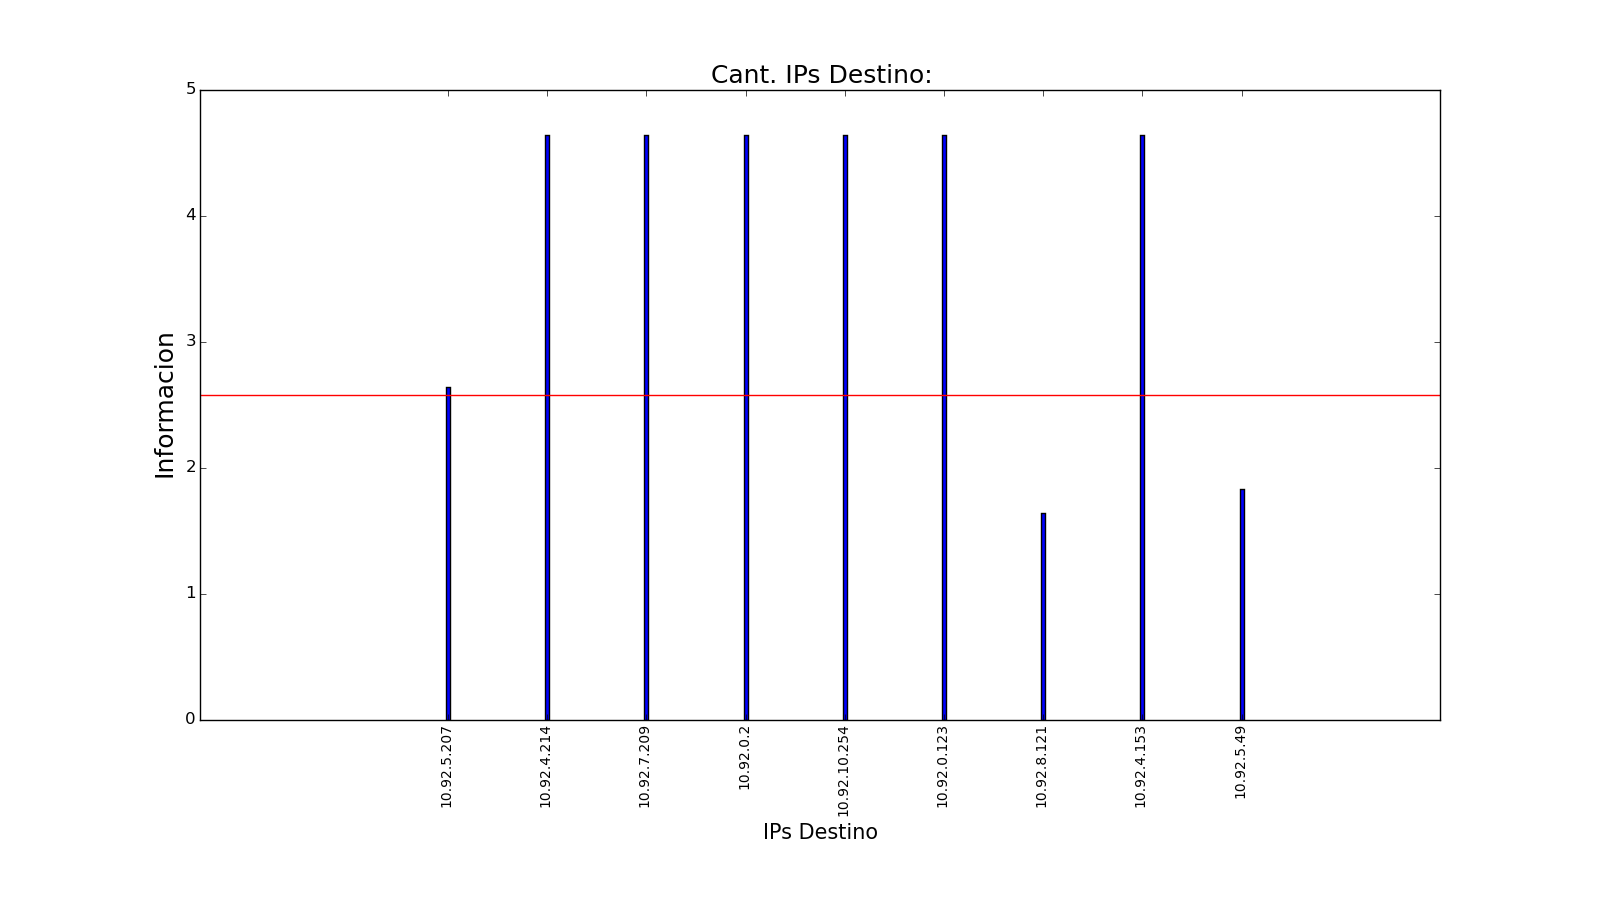
\includegraphics[width=1\textwidth]{../resultados/subte/histogram_dst_information.png}
       \caption{Información de IPs destino de los paquetes ARP}
       \label{red-Starbucks-dst-information}
\end{figure}

\begin{figure}[H]
       \centering
       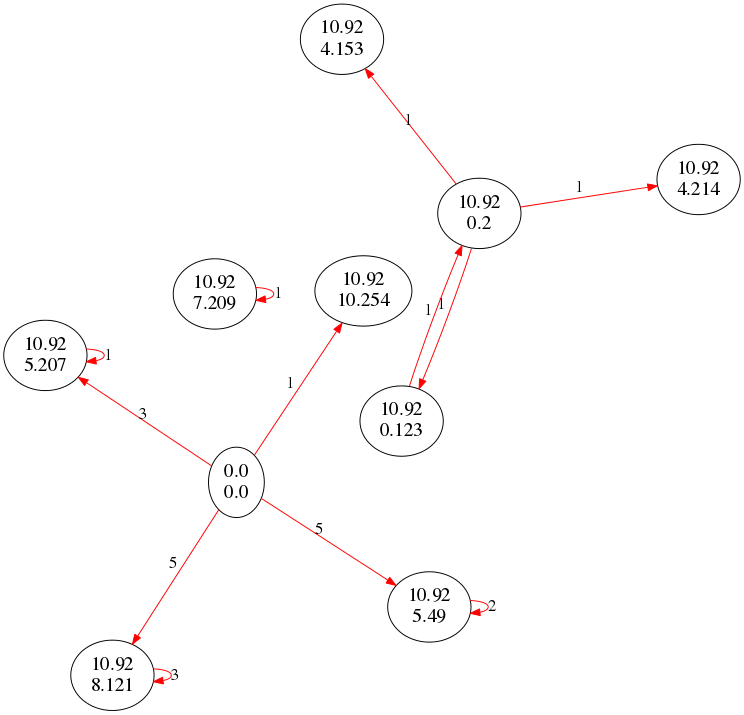
\includegraphics[width=1\textwidth]{../resultados/subte/network.png}
       \caption{Tráfico de paquetes ARP}
       \label{red-Starbucks-dst-information}
\end{figure}

Analizando los gráficos podemos ver que las IPs \textbf{10.92.8.121} y \textbf{10.92.5.49} reciben una mayor cantidad de paquetes que las demás y son nodos distinguidos por ser su información menor a la entropía. Pero los paquetes que reciben tienen como origen a la IP \textbf{0.0.0.0}, que como discutimos en la siguiente sección, son ARP requests que se mandan debido a la ejecución de un protocolo DHCP. No podemos sacar más conclusiones de estos gráficos debido al corto tiempo de intercepción de paquetes.\\
\newpage




\section{Resultados}

  \subsection{Red Hogareña}
  \subsubsection{Descripción y grafo de relación entre los nodos}

En este primer experimento, capturamos el tráfico de la LAN de un integrante de nuestro grupo. Medimos un Miércoles a las 00:00hs utilizando la red Wi-Fi. El tiempo de medición fue de aproximadamente 40 minutos, y capturamos aproximadamente 20 paquetes.

\begin{figure}[H]
  \begin{center}
    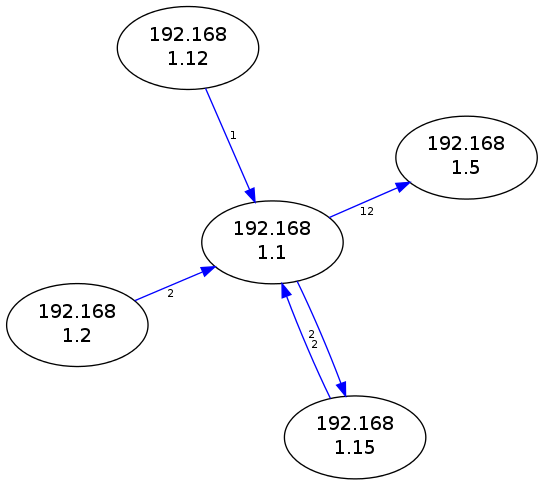
\includegraphics[width=0.3\linewidth]{../imgs/red-hogarena_red.png}
    \label{fig:FedeGrafo}
    \caption{Grafo de LAN hogareña}
  \end{center}
\end{figure}

\subsubsection{Fuente: $S_{dst}$}

\begin{figure}[H]\centering
    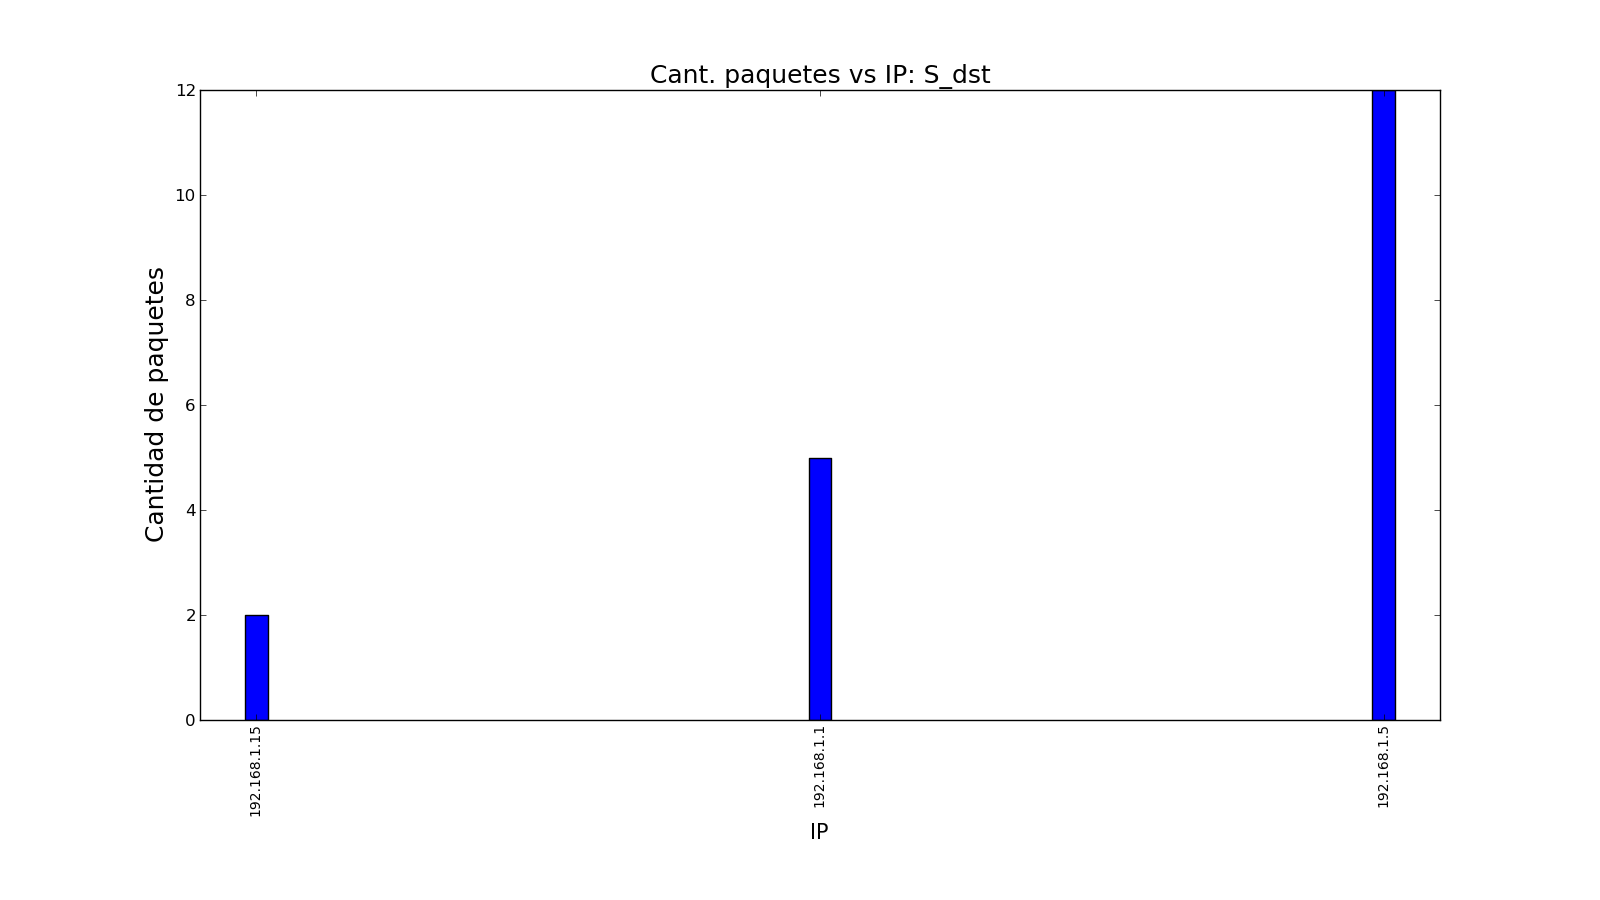
\includegraphics[width=0.8\linewidth]{../imgs/red-hogarena_S_dst_hist.png}
    \caption{Histograma de $S_{dst}$}\label{fig:Fede-dst-hist}
\end{figure}

\begin{figure}[H]\centering
    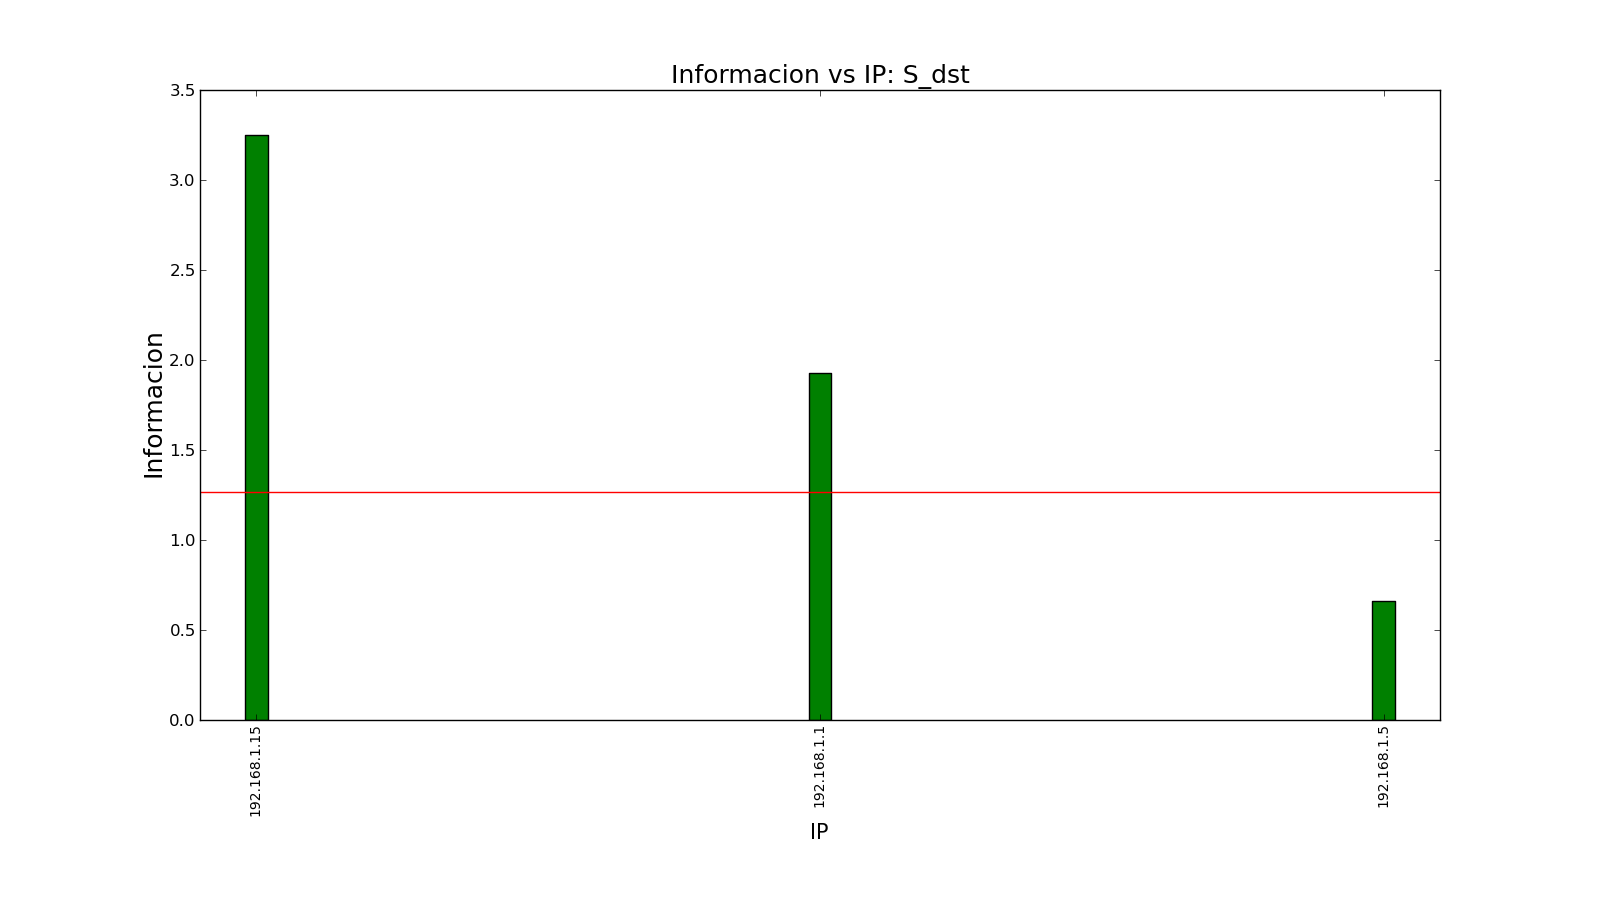
\includegraphics[width=0.8\linewidth]{../imgs/red-hogarena_S_dst_info.png}
    \caption{Informacion de $S_{dst}$}\label{fig:Fede-dst-info}
\end{figure}

$\bullet$ Entropía de la fuente: 1.26744380381

\subsubsection{Fuente: $S_{src}$}

\begin{figure}[H]\centering
    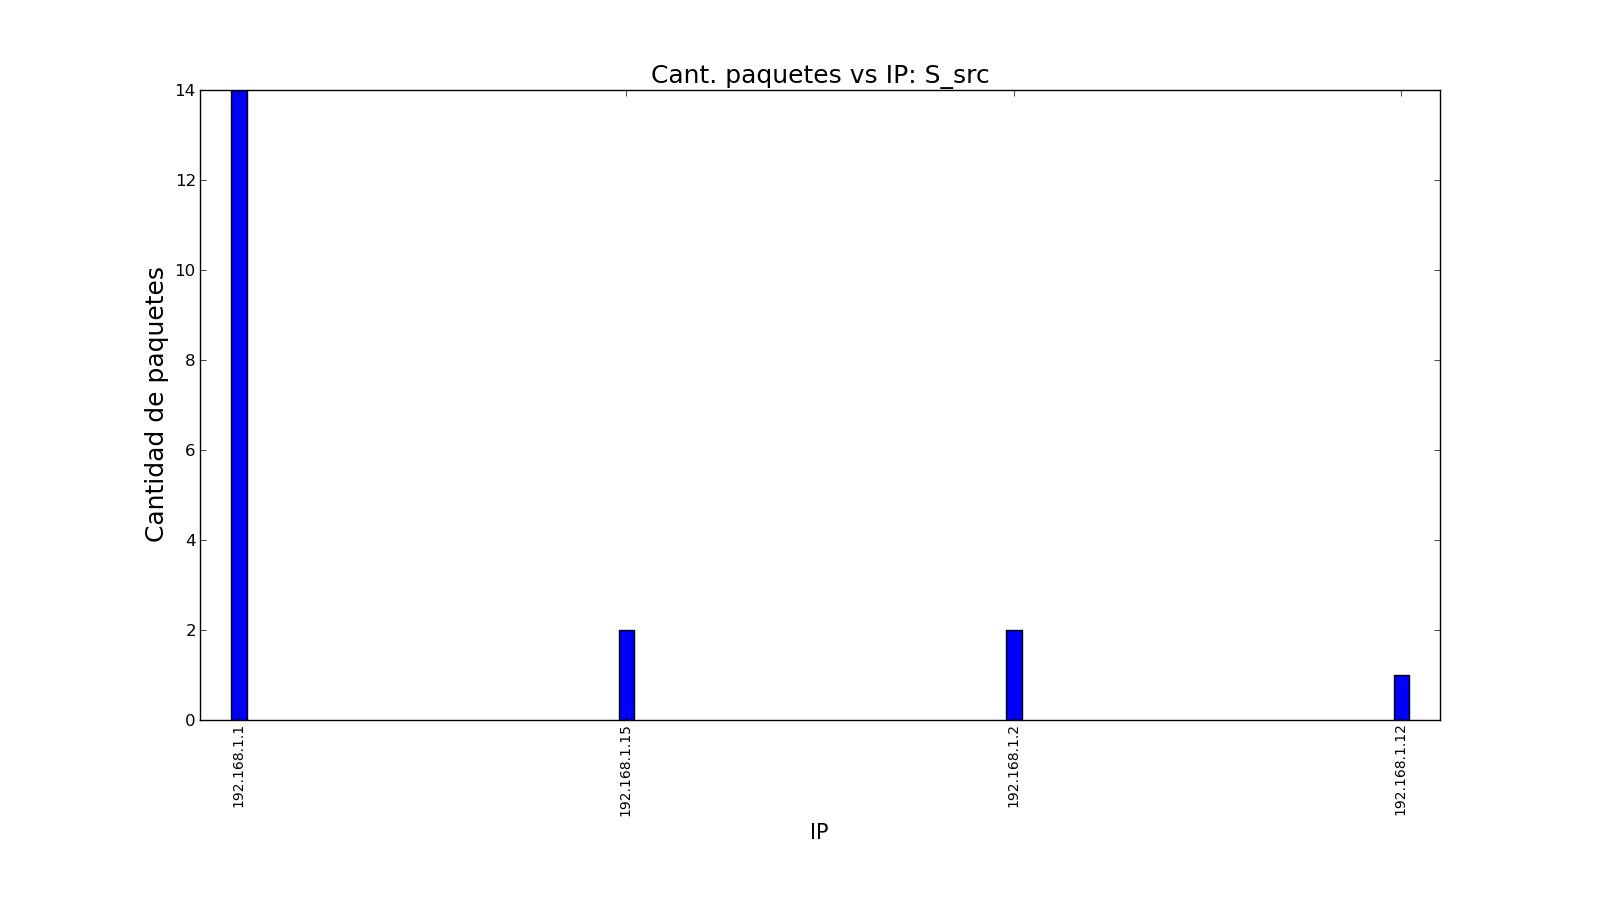
\includegraphics[width=0.8\linewidth]{../imgs/red-hogarena_S_src_hist.png}
    \caption{Histograma de $S_{src}$}\label{fig:Fede-src-hist}
\end{figure}

\begin{figure}[H]\centering
    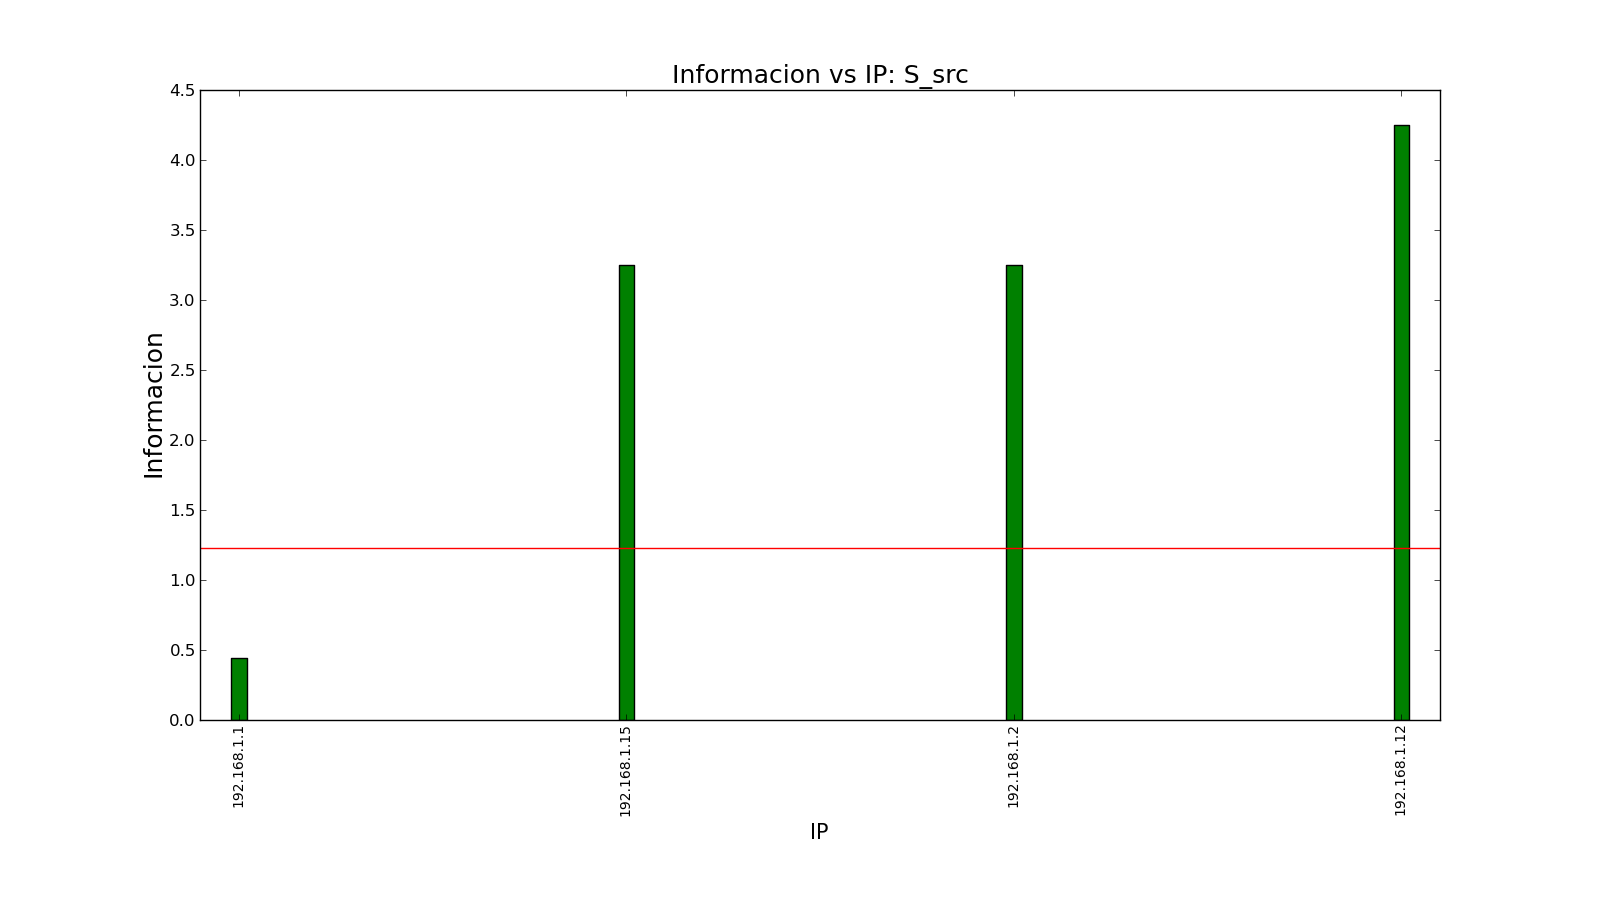
\includegraphics[width=0.8\linewidth]{../imgs/red-hogarena_S_src_info.png}
    \caption{Informacion de $S_{src}$}\label{fig:Fede-src-info}
\end{figure}

$\bullet$ Entropía de la fuente: 1.2319817814

\subsubsection{Discusión}

Debido a que es una red hogareña, tenemos una red bastante chica. En el grafo podemos observar un nodo (\emph{192.168.1.1}) el cual se conecta con todos los demás. A esta red la conocemos, y sabemos que dicho nodo es el router.

Como podemos observar en la Figura \ref{fig:Fede-src-info}, el router es un nodo distinguido en la fuente $S_{src}$. Sin embargo, en la Figura \ref{fig:Fede-dst-info} (fuente $S_{dst}$) el único nodo distinguido es \emph{192.168.1.5}. En el caso de \emph{192.168.1.5}, es una computadora que estaba bajando un archivo .torrent, y creemos que por eso 12 paquetes ARP \emph{who-has} tienen destino \emph{192.168.1.5}.

  \subsection{Red Alto Palermo}
  \subsubsection{Descripción y grafo de relación entre los nodos}

El siguiente experimento consistió en medir la LAN Wi-Fi pública del shopping Alto Palermo. Esta medición se llevó a cabo un día Sábado a las 21hs, con un tiempo de medición fue de aproximádamente 40 minutos y se capturaron 1569 paquetes ARP, de los cuales 687 eran de tipo \emph{who-has}.

A continuación mostramos un grafo que muestra los nodos de la red con su dirección IP y la cantidad de mensajes de tipo \emph{who-has}.

\begin{figure}[H]
 \begin{center}
  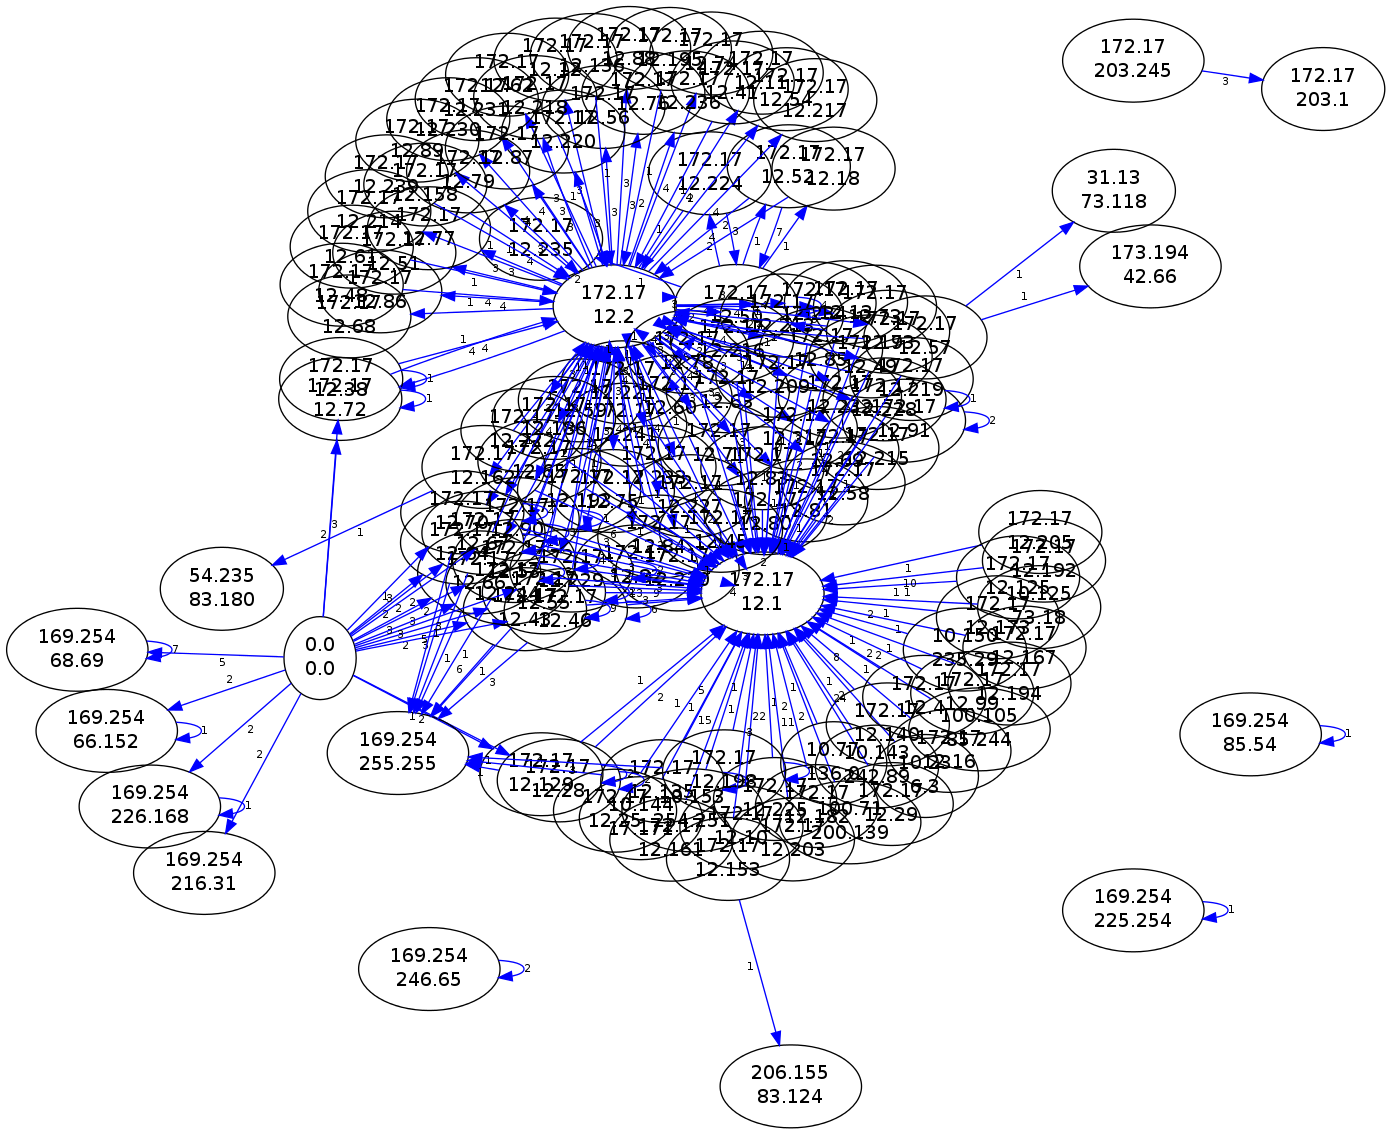
\includegraphics[width=0.9\linewidth]{../imgs/red-alto-palermo_red.png}
  \caption{Grafo Medición Alto Palermo}
 \end{center}
\end{figure}

Como podemos ver en el grafo, la red tiene dos nodos que se destacan. Uno de estos nodos, el cual tiene la dirección IP \emph{117.17.12.1}, recibe muchos paquetes de la mayoría de los otros nodos de la red, pero no envía ninguno. Y el otro, con dirección IP \emph{117.17.12.2} recibe varios paquetes y también envía varios.

También podemos observar que hay un nodo con dirección \emph{0.0.0.0}, el cual envía varios mensajes. %TODO explicar qué es el 0.0.0.0

\subsubsection{Fuente: $S_{dst}$}

A continuación incluimos el histograma y el gráfico de información de la fuente $S_{dst}$. 

\begin{figure}[H]\centering
  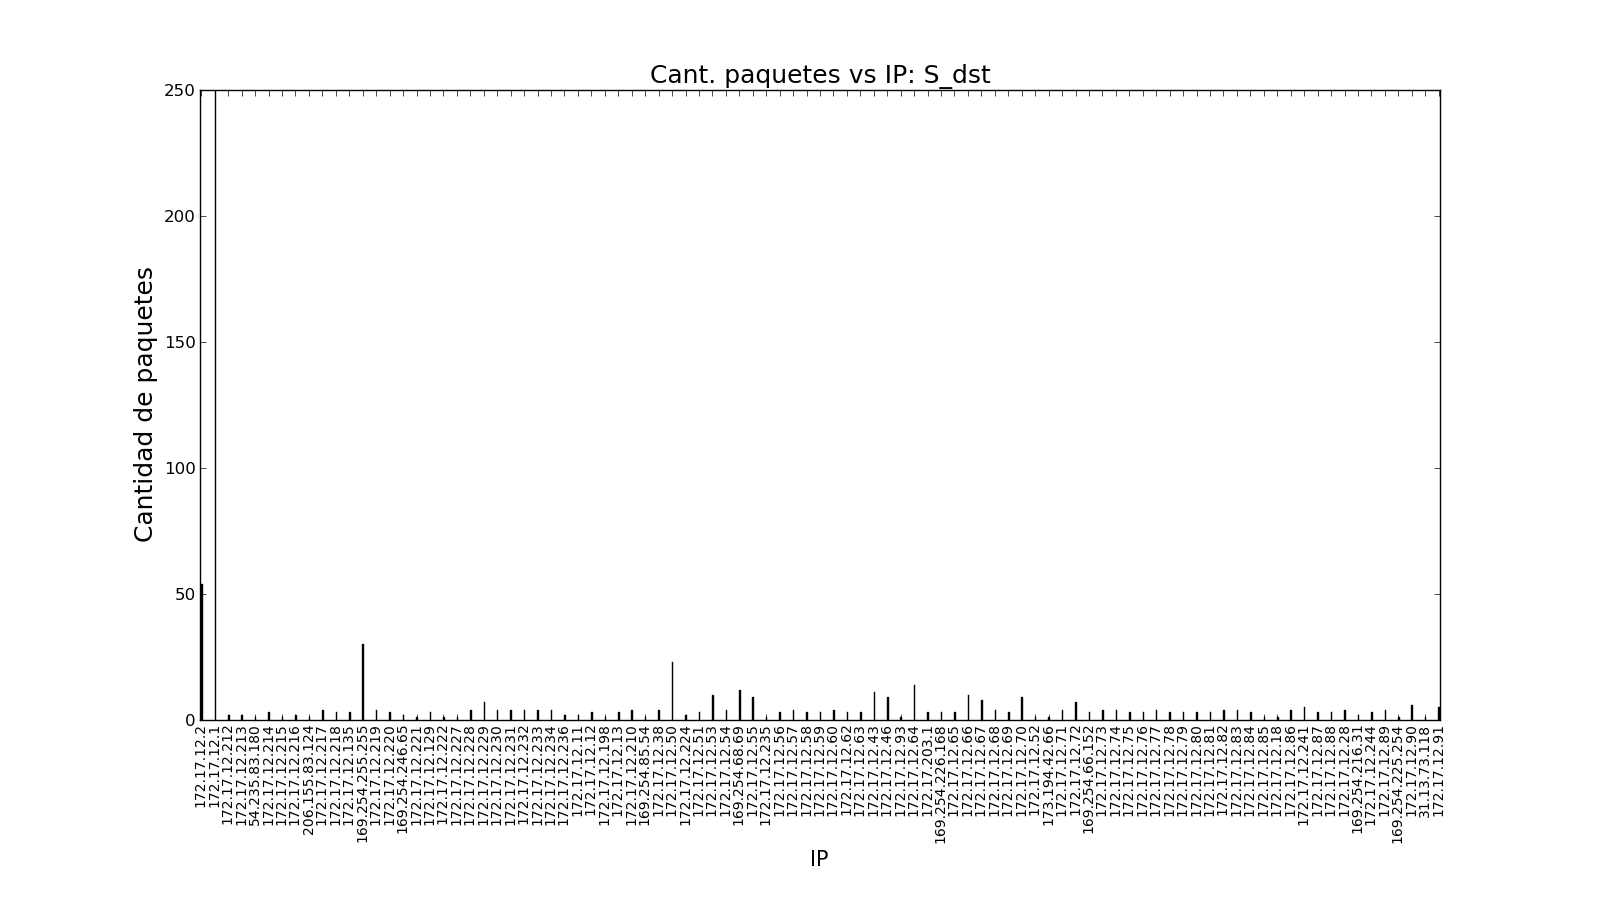
\includegraphics[width=0.8\linewidth]{../imgs/red-alto-palermo_S_dst_hist.png}
  \caption{Histograma de $S_{dst}$}\label{fig:Alto-dst-hist}
\end{figure}

\begin{figure}[H]\centering
  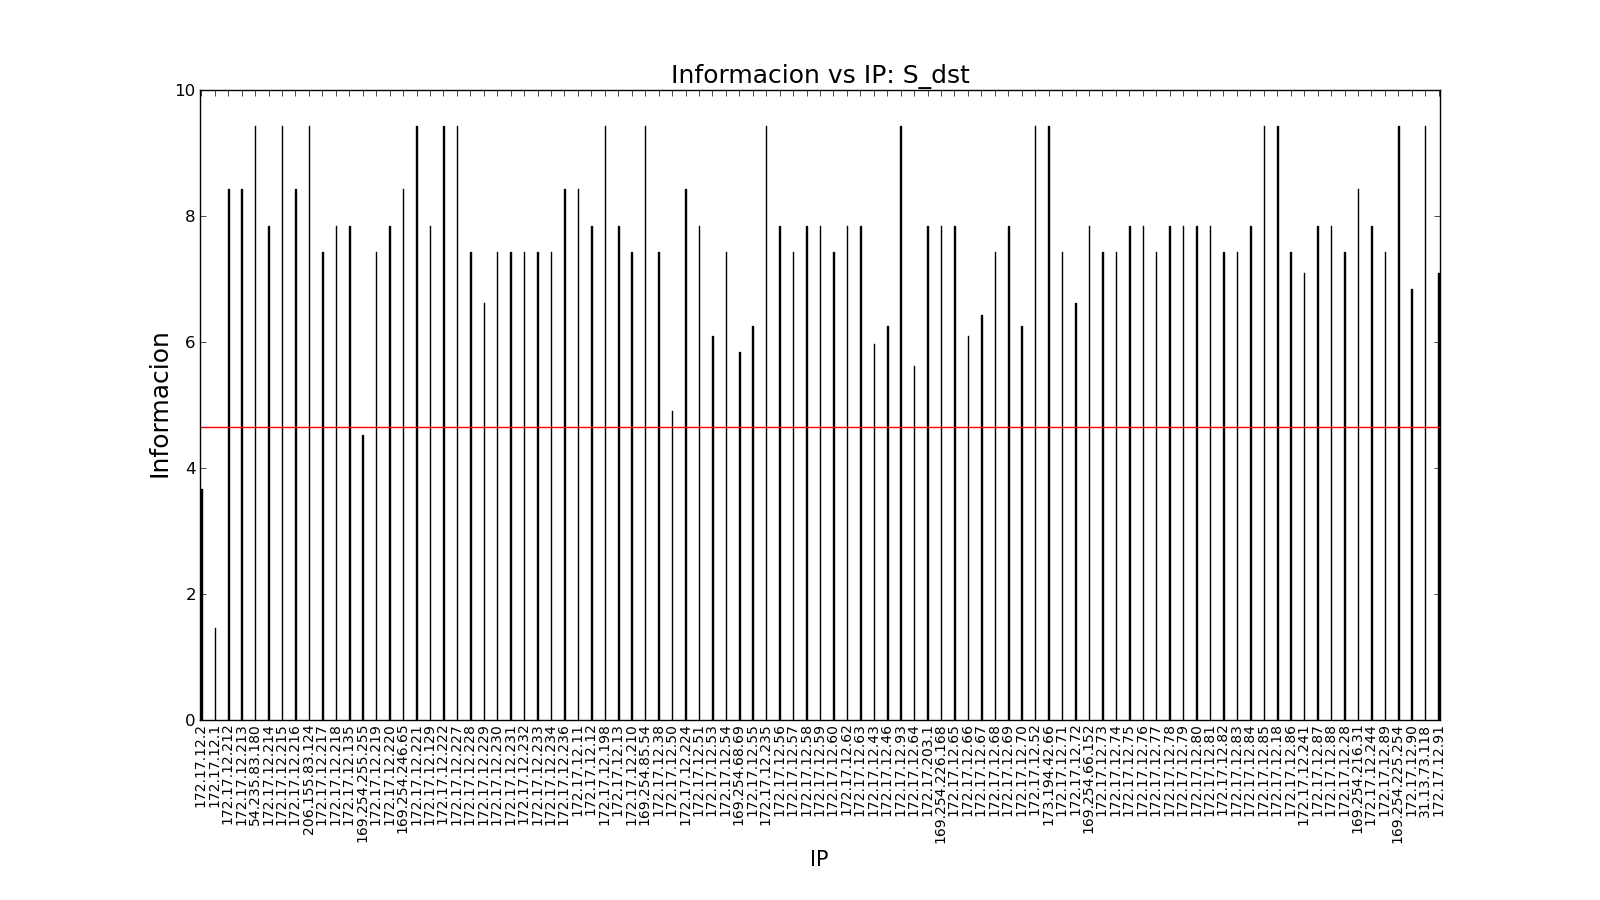
\includegraphics[width=0.8\linewidth]{../imgs/red-alto-palermo_S_dst_info.png}
  \caption{Informacion de $S_{dst}$}\label{fig:Alto-dst-info}
\end{figure}

$\bullet$ Entropía de la fuente: 4.65701881033

Como podemos observar en el primer gráfico, la dirección IP \emph{172.17.12.1} aparece muchas más veces que el resto de las IP. Esto es así porque dicha dirección recibe mensajes de casi todos los demás nodos de la red. Los nodos con direcciónes \emph{172.17.12.2} y \emph{169.254.255.255} también se destacan en el gráfico.

En el segundo gráfico podemos ver que la cantidad de información que aporta la dirección IP \emph{177.17.12.1} es más baja que la entopía de la fuente, al igual que la de las direcciones \emph{172.17.12.2} y \emph{169.254.255.255}.

\subsubsection{Fuente: $S_{src}$}

A contincuación mostramos gráficos similares, pero esta vez para la fuente $S_{src}$:

\begin{figure}[H]\centering
    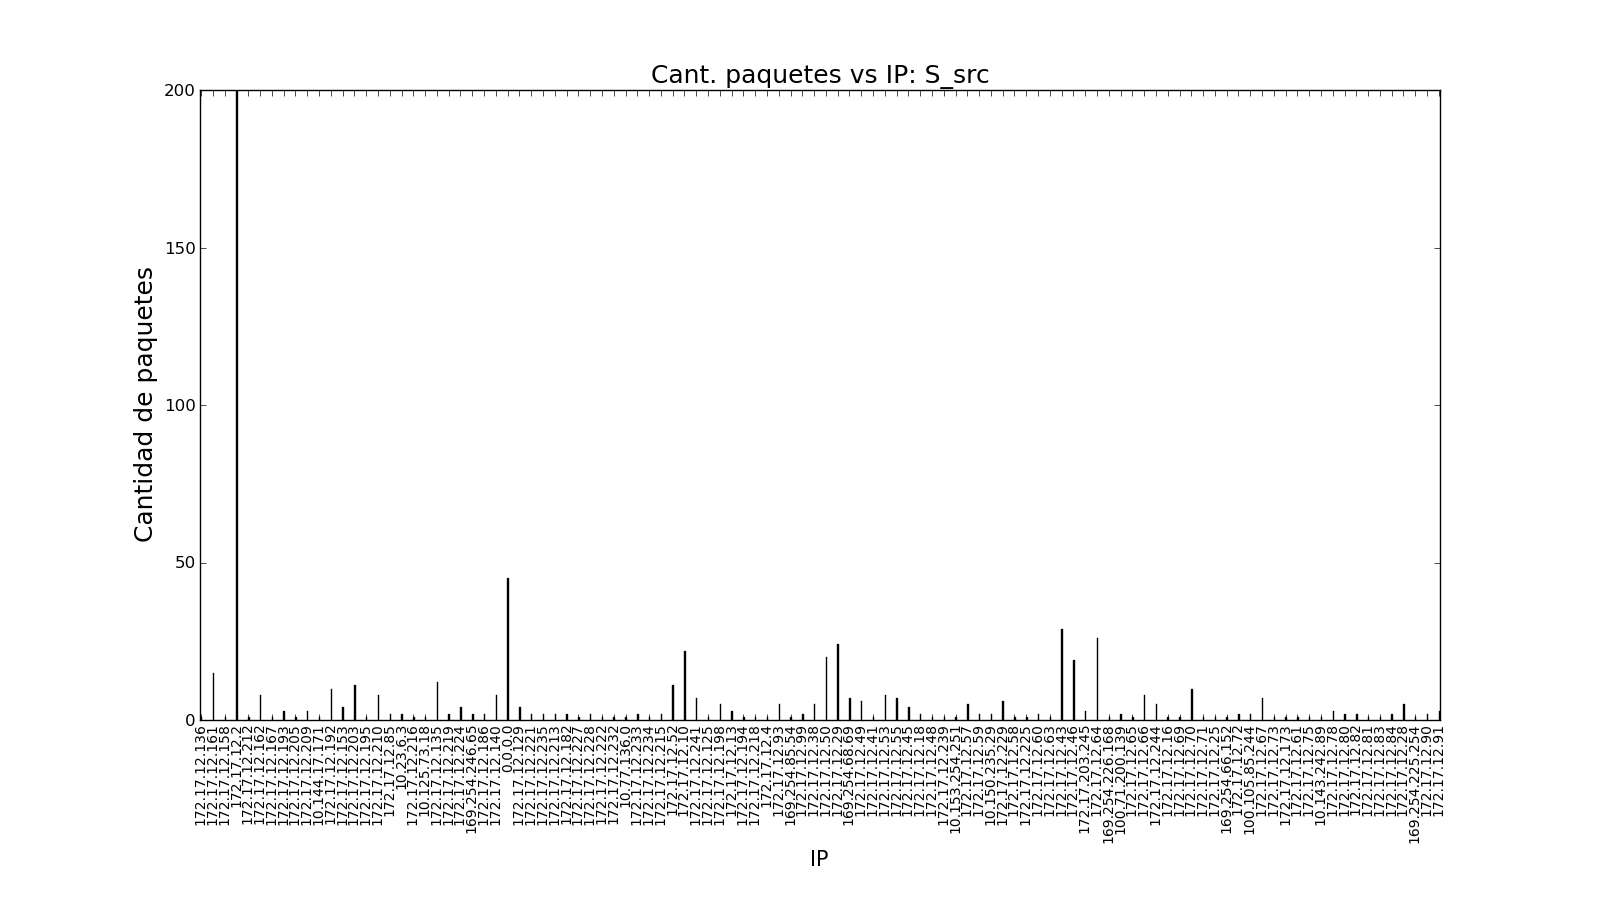
\includegraphics[width=0.8\linewidth]{../imgs/red-alto-palermo_S_src_hist.png}
    \caption{Histograma de $S_{src}$}\label{fig:Alto-src-hist}
\end{figure}

\begin{figure}[H]\centering
    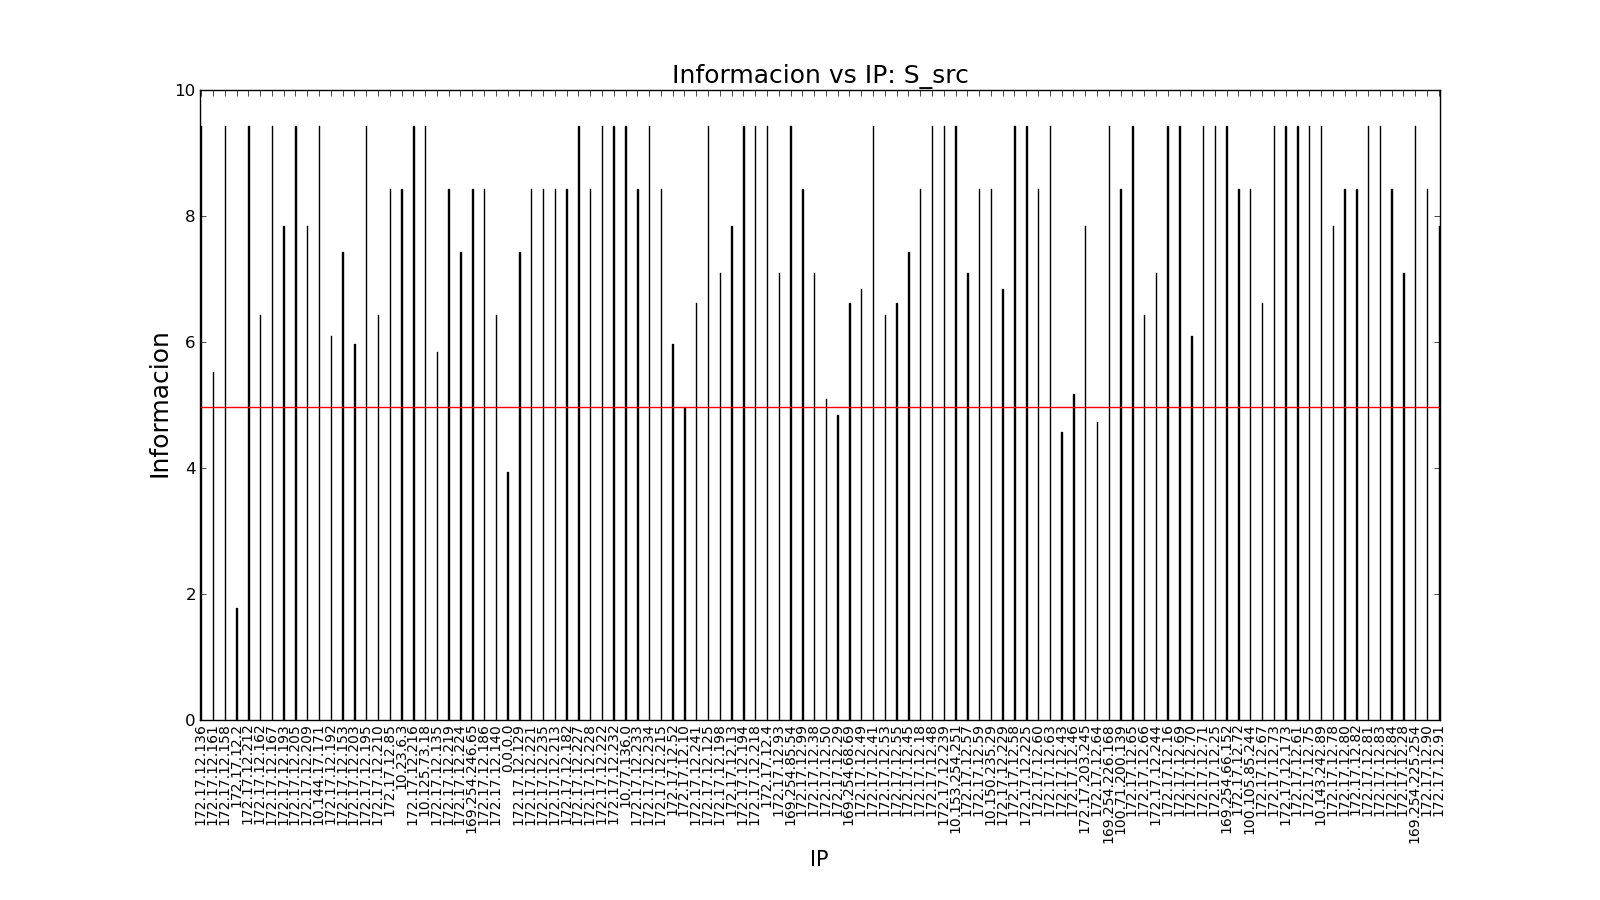
\includegraphics[width=0.8\linewidth]{../imgs/red-alto-palermo_S_src_info.png}
    \caption{Informacion de $S_{src}$}\label{fig:Alto-src-info}
\end{figure}

$\bullet$ Entropía de la fuente: 4.96088403083

En el segundo gráfico podemos observar que hay 5 nodos que aportan menos información que la entropía de la fuente. Estos tienen las direciones \emph{172.17.12.1}, \emph{172.17.12.45}, \emph{172.17.12.64}, \emph{172.17.12.29} y la \emph{0.0.0.0}. 

En el primer gráfico podemos observar que el nodo que tiene la dirección IP \emph{172.17.12.2} envía muchos más paquetes que el resto de los nodos. 

\subsubsection{Discusión}

Suponemos que la dirección \emph{172.17.12.1} es el router de la red ya que es el que aparece como dirección destino en la mayor parte de paquetes \emph{who-has}. Algo que nos llamó la atención es que aparece la dirección \emph{0.0.0.0} como dirección fuente en varios mensajes. Lamentablemente no pudimos saber a que se debe esto.
Además creemos que la dirección \emph{169.254.255.255} es una dirección \emph{broadcast}, ya que su dirección termina con 255.255 y aparece como dirección destino en muchos paquetes (es un nodo distinguido de la fuente $S_{dst}$.
Sin embargo, no pudimos ver qué rol ocupa el nodo con dirección \emph{172.17.12.2}

% %
% Cuando observamos el grafo en la primera parte del análisis de esta red, dijimos que había dos nodos que se destacaban visualmente, los cuales eran los que tenían las direcciones IP \emph{172.17.12.1} y \emph{172.17.12.2}. Al ver el grafo notamos que la mayor parte de los paquetes capturados eran enviados o recibidos por alguno de estos dos nodos. Esto nos hizo suponer que éstos eran dos nodos distinguidos de la red.
% 
% Luego observamos el histograma y el gráfico de barras de la fuente $S_{dst}$. De esta forma vimos que efectivamente el nodo con la IP \emph{172.17.12.1} aparecía como dirección destino en muchos mensajes. Sin embargo el nodo \emph{172.17.12.2} no aparecía tantas veces.
% 
% Al hacer lo mismo con la fuente $S_{src}$ notamos que el nodo que aparecía más veces era el nodo \emph{172.17.12.2}. El nodo \emph{172.17.12.1} no era un símbolo de $S_{src}$ ya que éste no mandó mensajes, por lo tanto no aparece en estos gráficos.
% 
% Concluimos entonces que el nodo de la red que tiene la dirección IP \emph{172.17.12.1} se trata de un nodo distinguido, el cual creemos que es el router de la red. Sin embargo, no pudimos ver qué rol ocupaba el nodo \emph{172.17.12.2} en la misma.

  \subsection{Red Honeywell}
  \subsubsection{Descripción y grafo de relación entre los nodos}

Este experimento consistió en capturar los paquetes de la LAN Wi-Fi de la empresa Honeywell. En esta red no hay mucho tráfico, ya que la mayoría de las computadoras se conectan via Ethernet a una VPN. Esta red es dedicada a transacciones que no necesiten un nivel de seguridad (para uso de teléfonos celulares más que nada). La captura se realizo un día lunes a las 11 am. durante media hora, lográndose capturar 253 paquetes.  

\begin{figure}[H]
 \begin{center}
  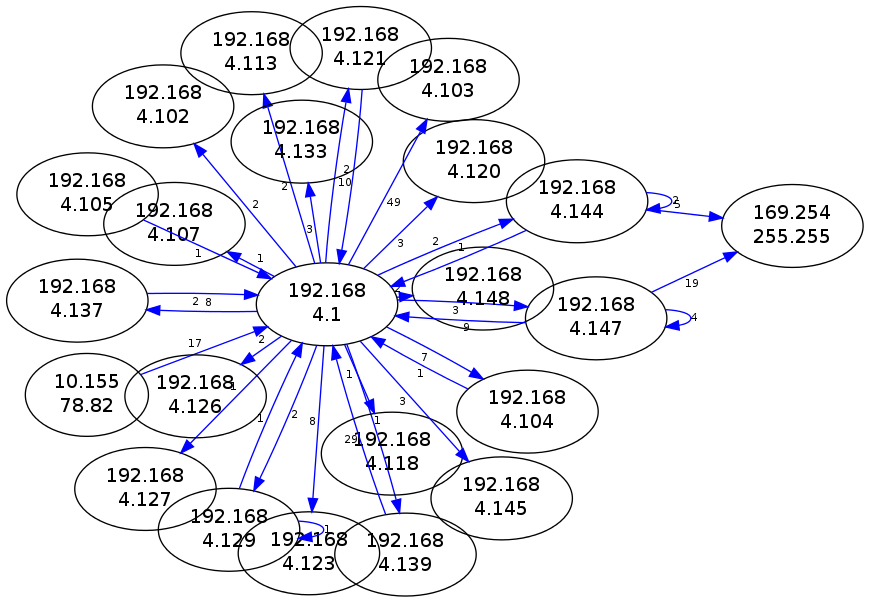
\includegraphics[width=0.7\linewidth]{../imgs/red-honeywell_red.png}
  \caption{Medición Honeywell}
 \end{center}
\end{figure}

El primer nodo que se destaca a simple vista es el \emph{192.168.4.1}, que es el \emph{src} o \emph{dst} de casi todo paquete encontrado.
También distinguimos \emph{169.254.255.255} ya que es el único nodo que no es vecino de \emph{192.168.4.1}.

\subsubsection{Fuente: $S_{dst}$}

\begin{figure}[H]\centering
    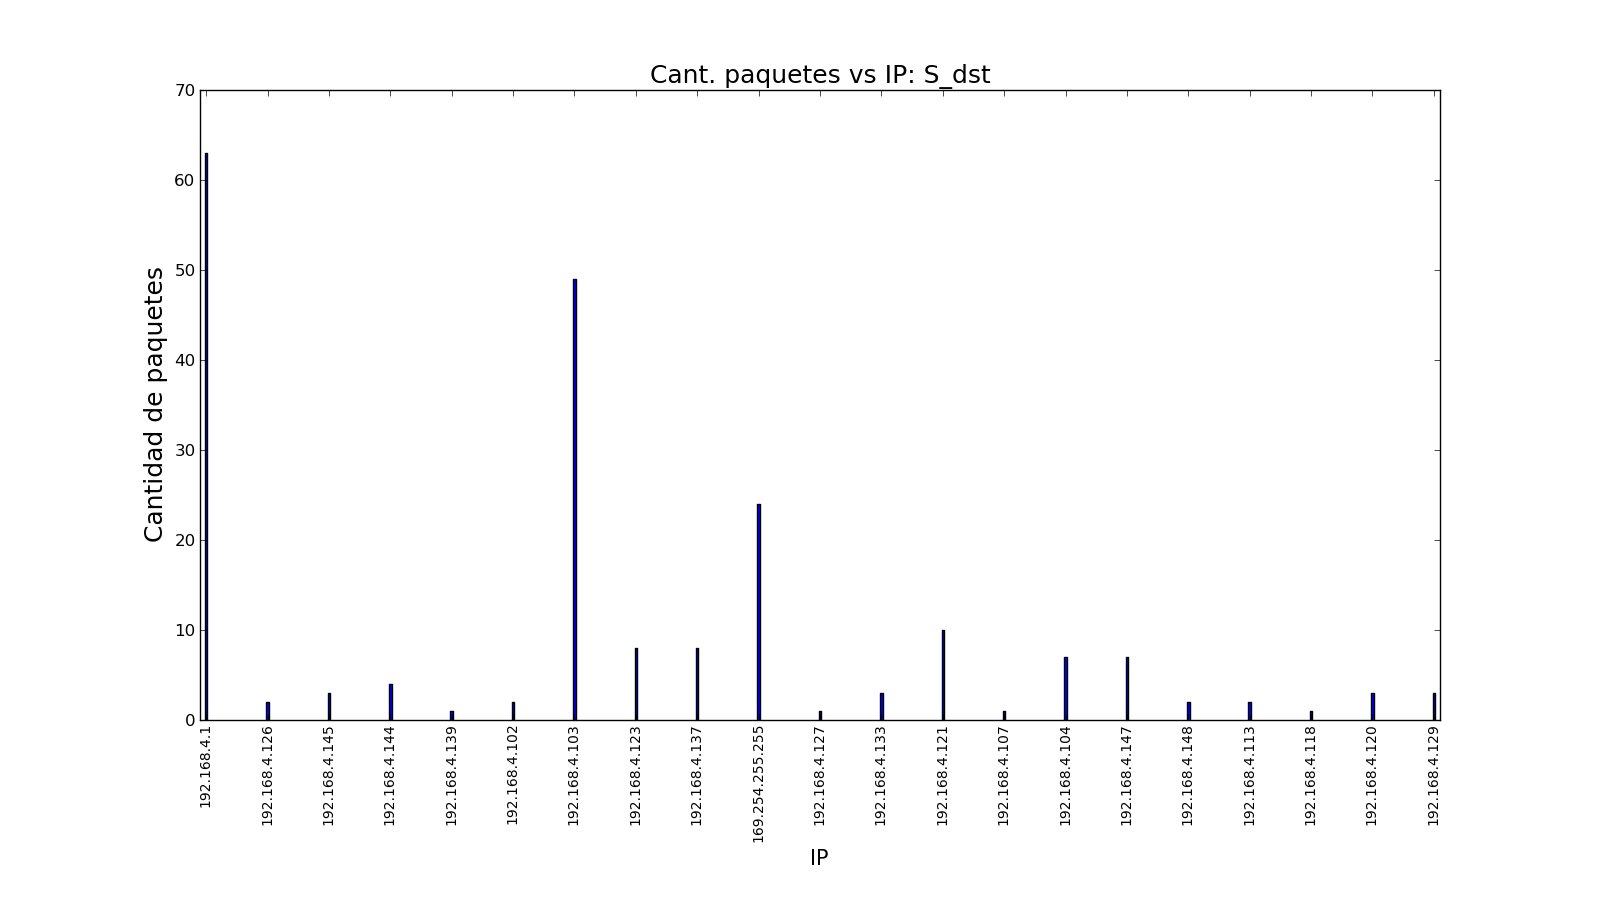
\includegraphics[width=0.8\linewidth]{../imgs/red-honeywell_S_dst_hist.png}
    \caption{Histograma de $S_{dst}$}\label{fig:Honeywell-dst-hist}
\end{figure}

\begin{figure}[H]\centering
    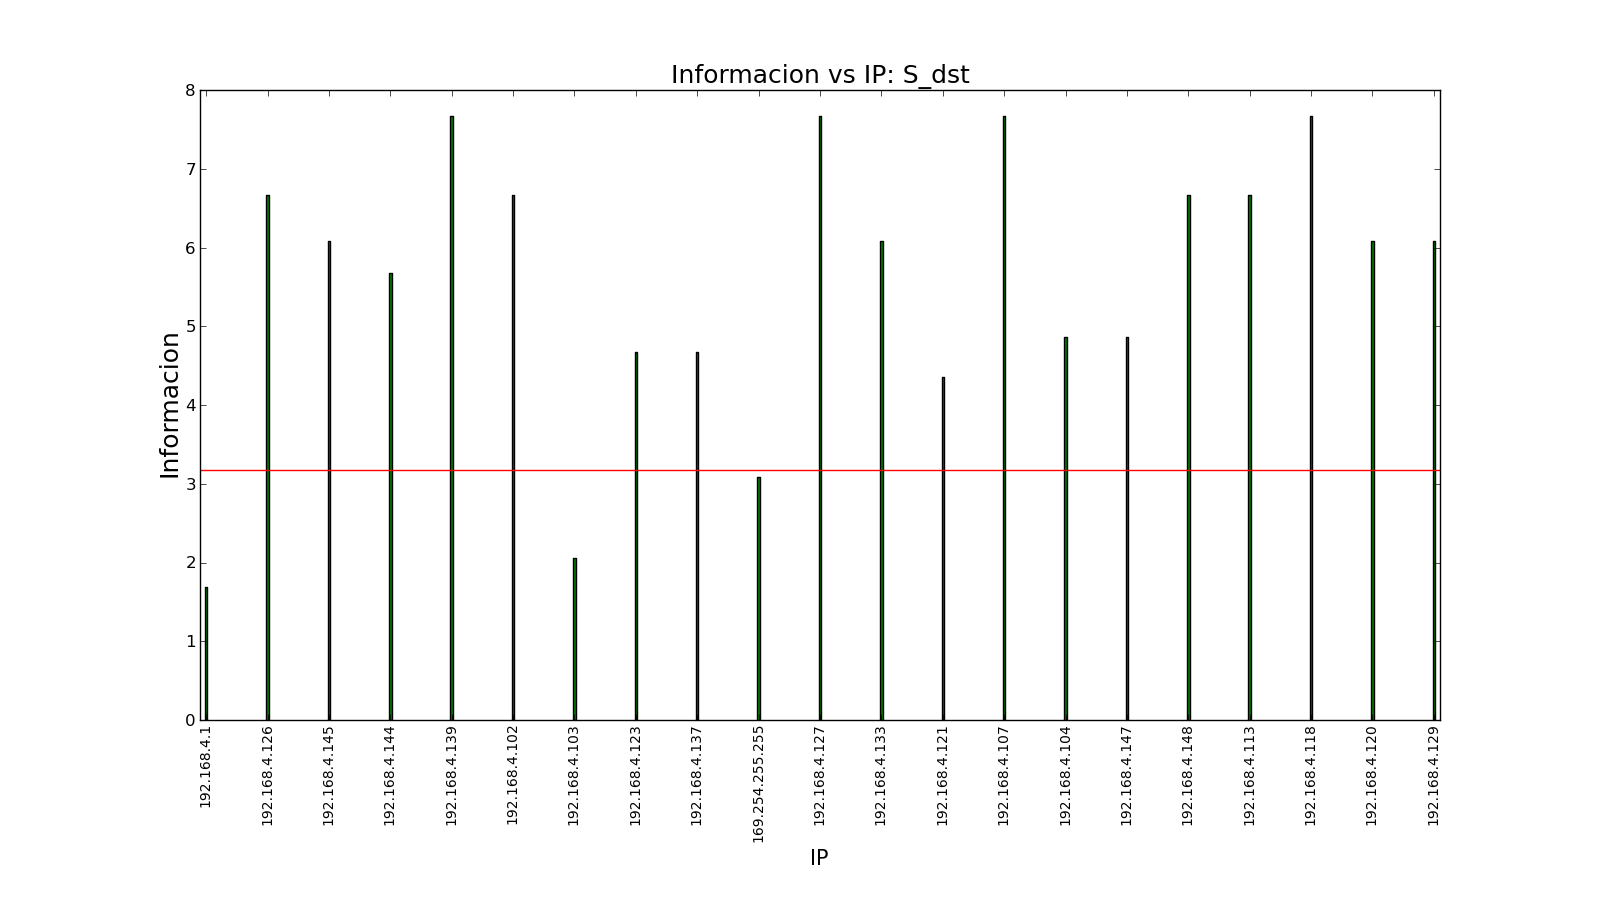
\includegraphics[width=0.8\linewidth]{../imgs/red-honeywell_S_dst_info.png}
    \caption{Informacion de $S_{dst}$}\label{fig:Honeywell-dst-info}
\end{figure}
En la Figura \ref{fig:Honeywell-dst-hist} podemos ver 3 nodos visualmente distinguibles, \emph{192.168.4.1}, \emph{192.168.4.103} y \emph{169.254.255.255}.
Cuando analizamos la Figura \ref{fig:Honeywell-dst-info}, podemos corroborar que estos nodos son distinguidos, ya que su información es menor a la entropía de la fuente.

$\bullet$ Entropía de la fuente: 3.17600221734

\subsubsection{Fuente: $S_{src}$}

\begin{figure}[H]\centering
    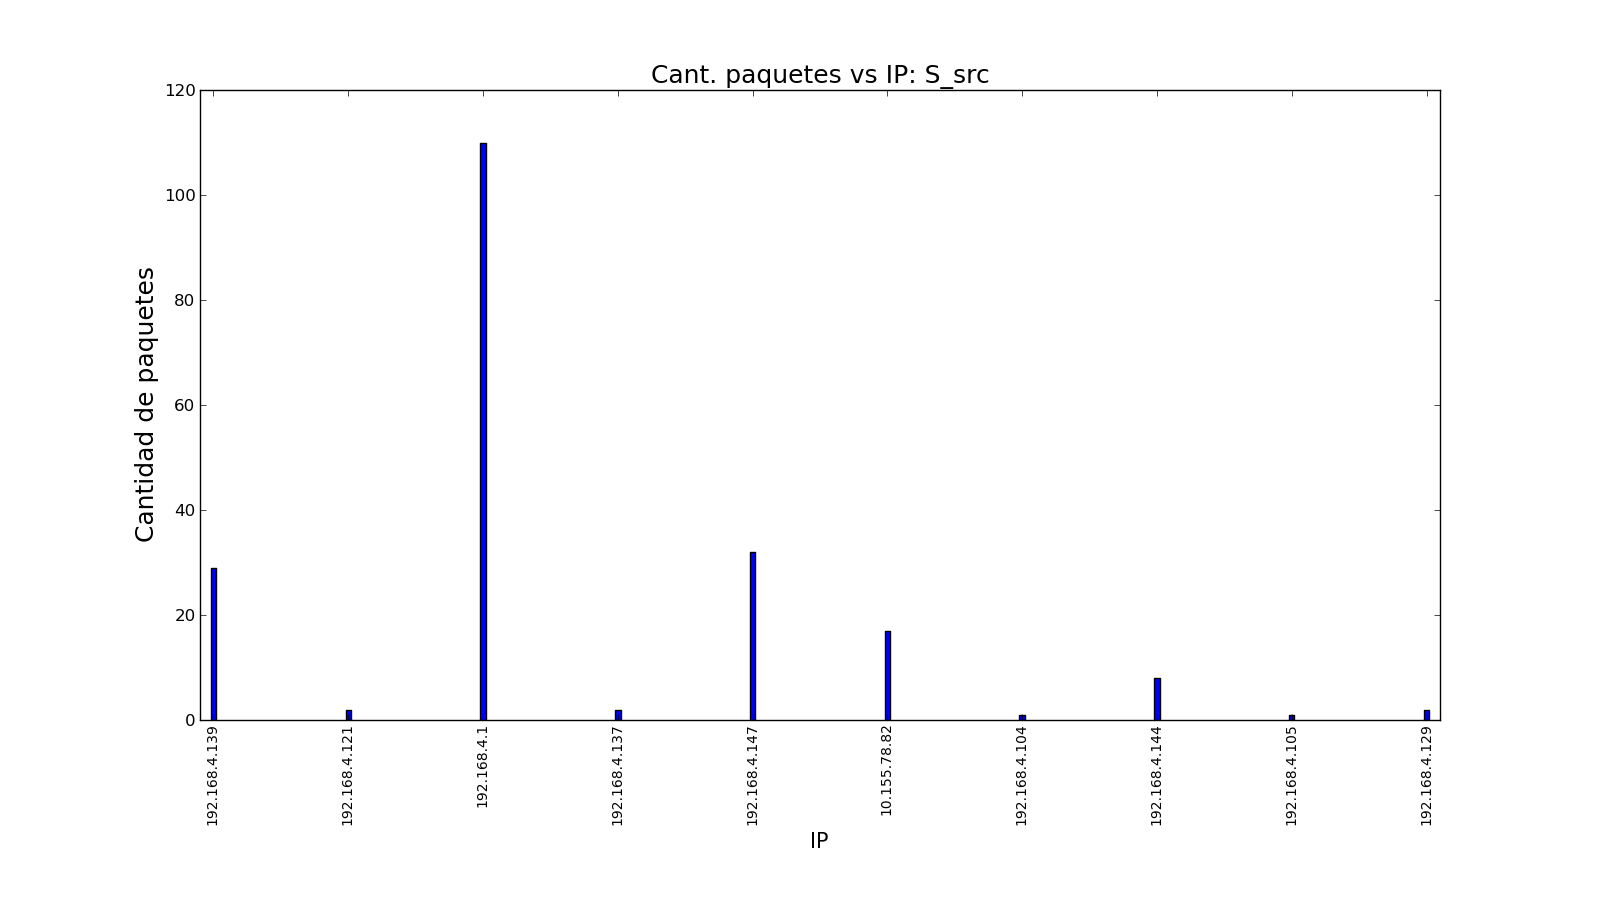
\includegraphics[width=0.8\linewidth]{../imgs/red-honeywell_S_src_hist.png}
    \caption{Histograma de $S_{src}$}\label{fig:Honeywell-src-hist}
\end{figure}

\begin{figure}[H]\centering
    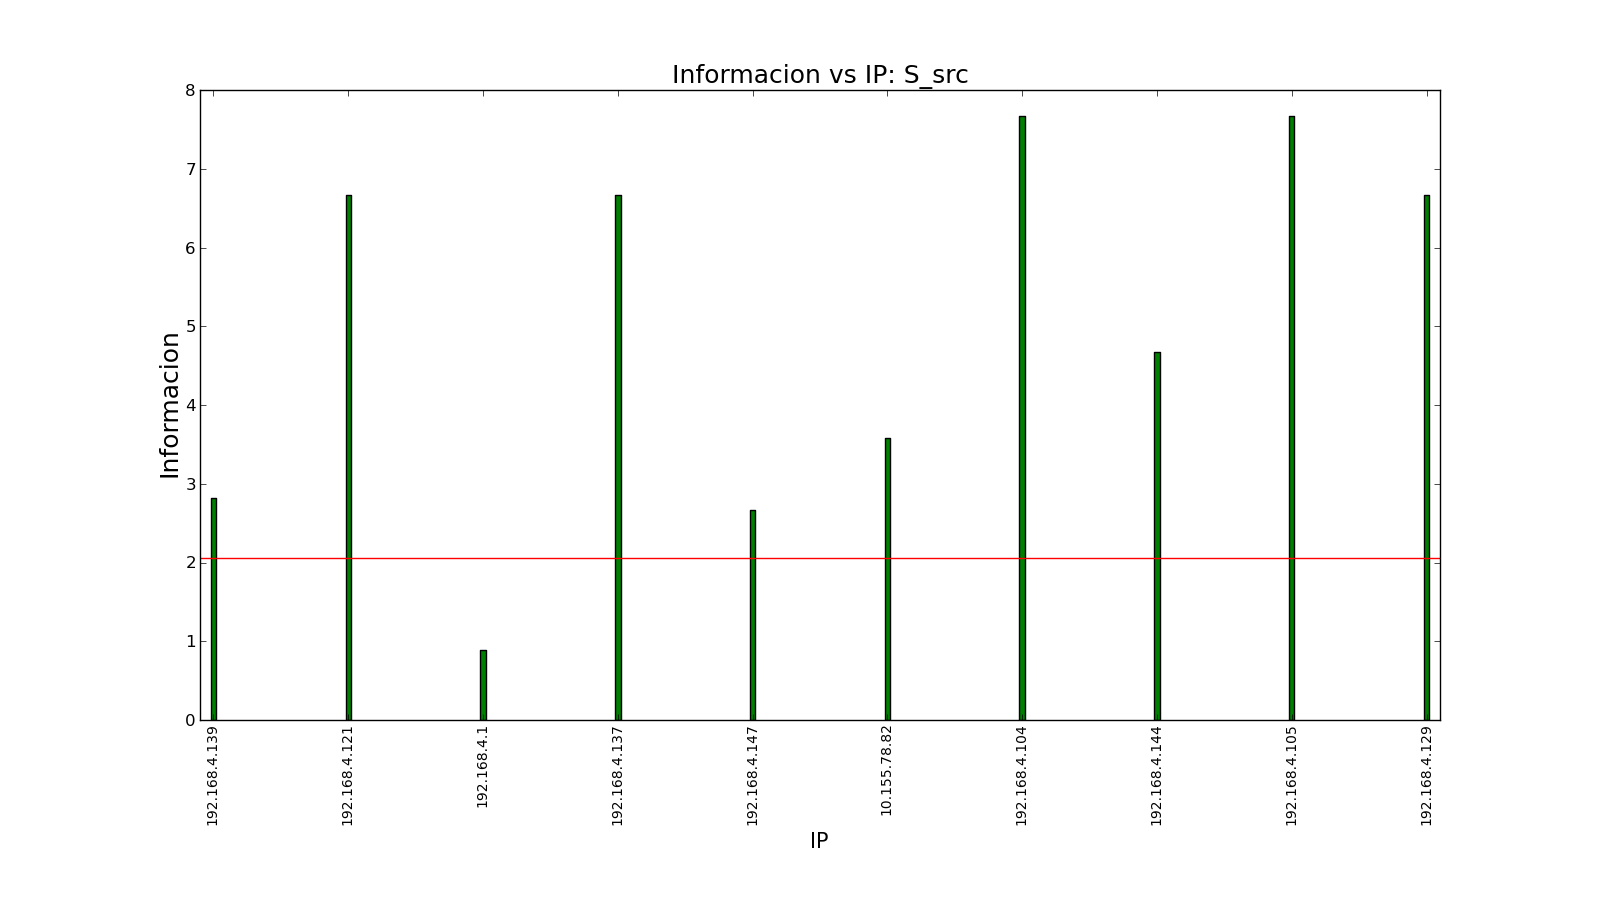
\includegraphics[width=0.8\linewidth]{../imgs/red-honeywell_S_src_info.png}
    \caption{Informacion de $S_{src}$}\label{fig:Honeywell-src-info}
\end{figure}

En la Figura \ref{fig:Honeywell-src-hist} podemos ver un nodo visualmente distinguible, \emph{192.168.4.1}.
Cuando analizamos la Figura \ref{fig:Honeywell-src-info}, podemos corroborar que este nodo es distinguido, ya que su información es menor a la entropía de la fuente.

$\bullet$ Entropía de la fuente: 2.05322002017



\subsubsection{Discusión}

Suponemos que \emph{192.168.4.1} es el router de la red, ya que no solo es un nodo distinguido, sino que vemos en la red que tiene transacciones con casi todos los nodos de la red.
Suponemos que \emph{169.254.255.255} suponemos que es una dirección de \emph{broadcast}, ya que no solo termina con 255.255 (dieciséis 1 en binario), sino que además tiene alta probabilidad como \emph{dst} pero nunca aparece como \emph{src}.
Suponemos que \emph{192.168.4.103} es una terminal con un alto acceso a internet en el momento de la medición (descarga), ya que es un nodo destacado como \emph{dst}, pero no aparece como \emph{src}. Y todos la paquetes los recibe de \emph{192.168.4.1} (que supusimos es el router). 


  \subsection{Red Laboratorios DC}
  \subsubsection{Descripción y grafo de relación entre los nodos}

Realizamos una captura en la red Wi-Fi \emph{Entrepiso-DC}, disponible desde los laboratorios del Depto. de Computación. La muestra fue tomada un lunes a las 17hs aproximadamente -horario típicamente de alto tráfico-, logrando un total de 450 paquetes en 11 minutos.

En el gráfico de la figura \ref{fig:entrepiso-dc-grafo} se presenta el grafo dirigido representando la red. En el mismo se observa una gran cantidad de nodos ligada al nodo con IP \emph{10.1.200.197}, y luego múltiples conjuntos pequeños de nodos conectados entre sí pero disconexos de la estructura mayoritaria. Es decir, a diferencia de las demás redes observadas, esta presentó una gran cantidad de pequeños clusters independientes.

\begin{figure}[H]
  \begin{center}
    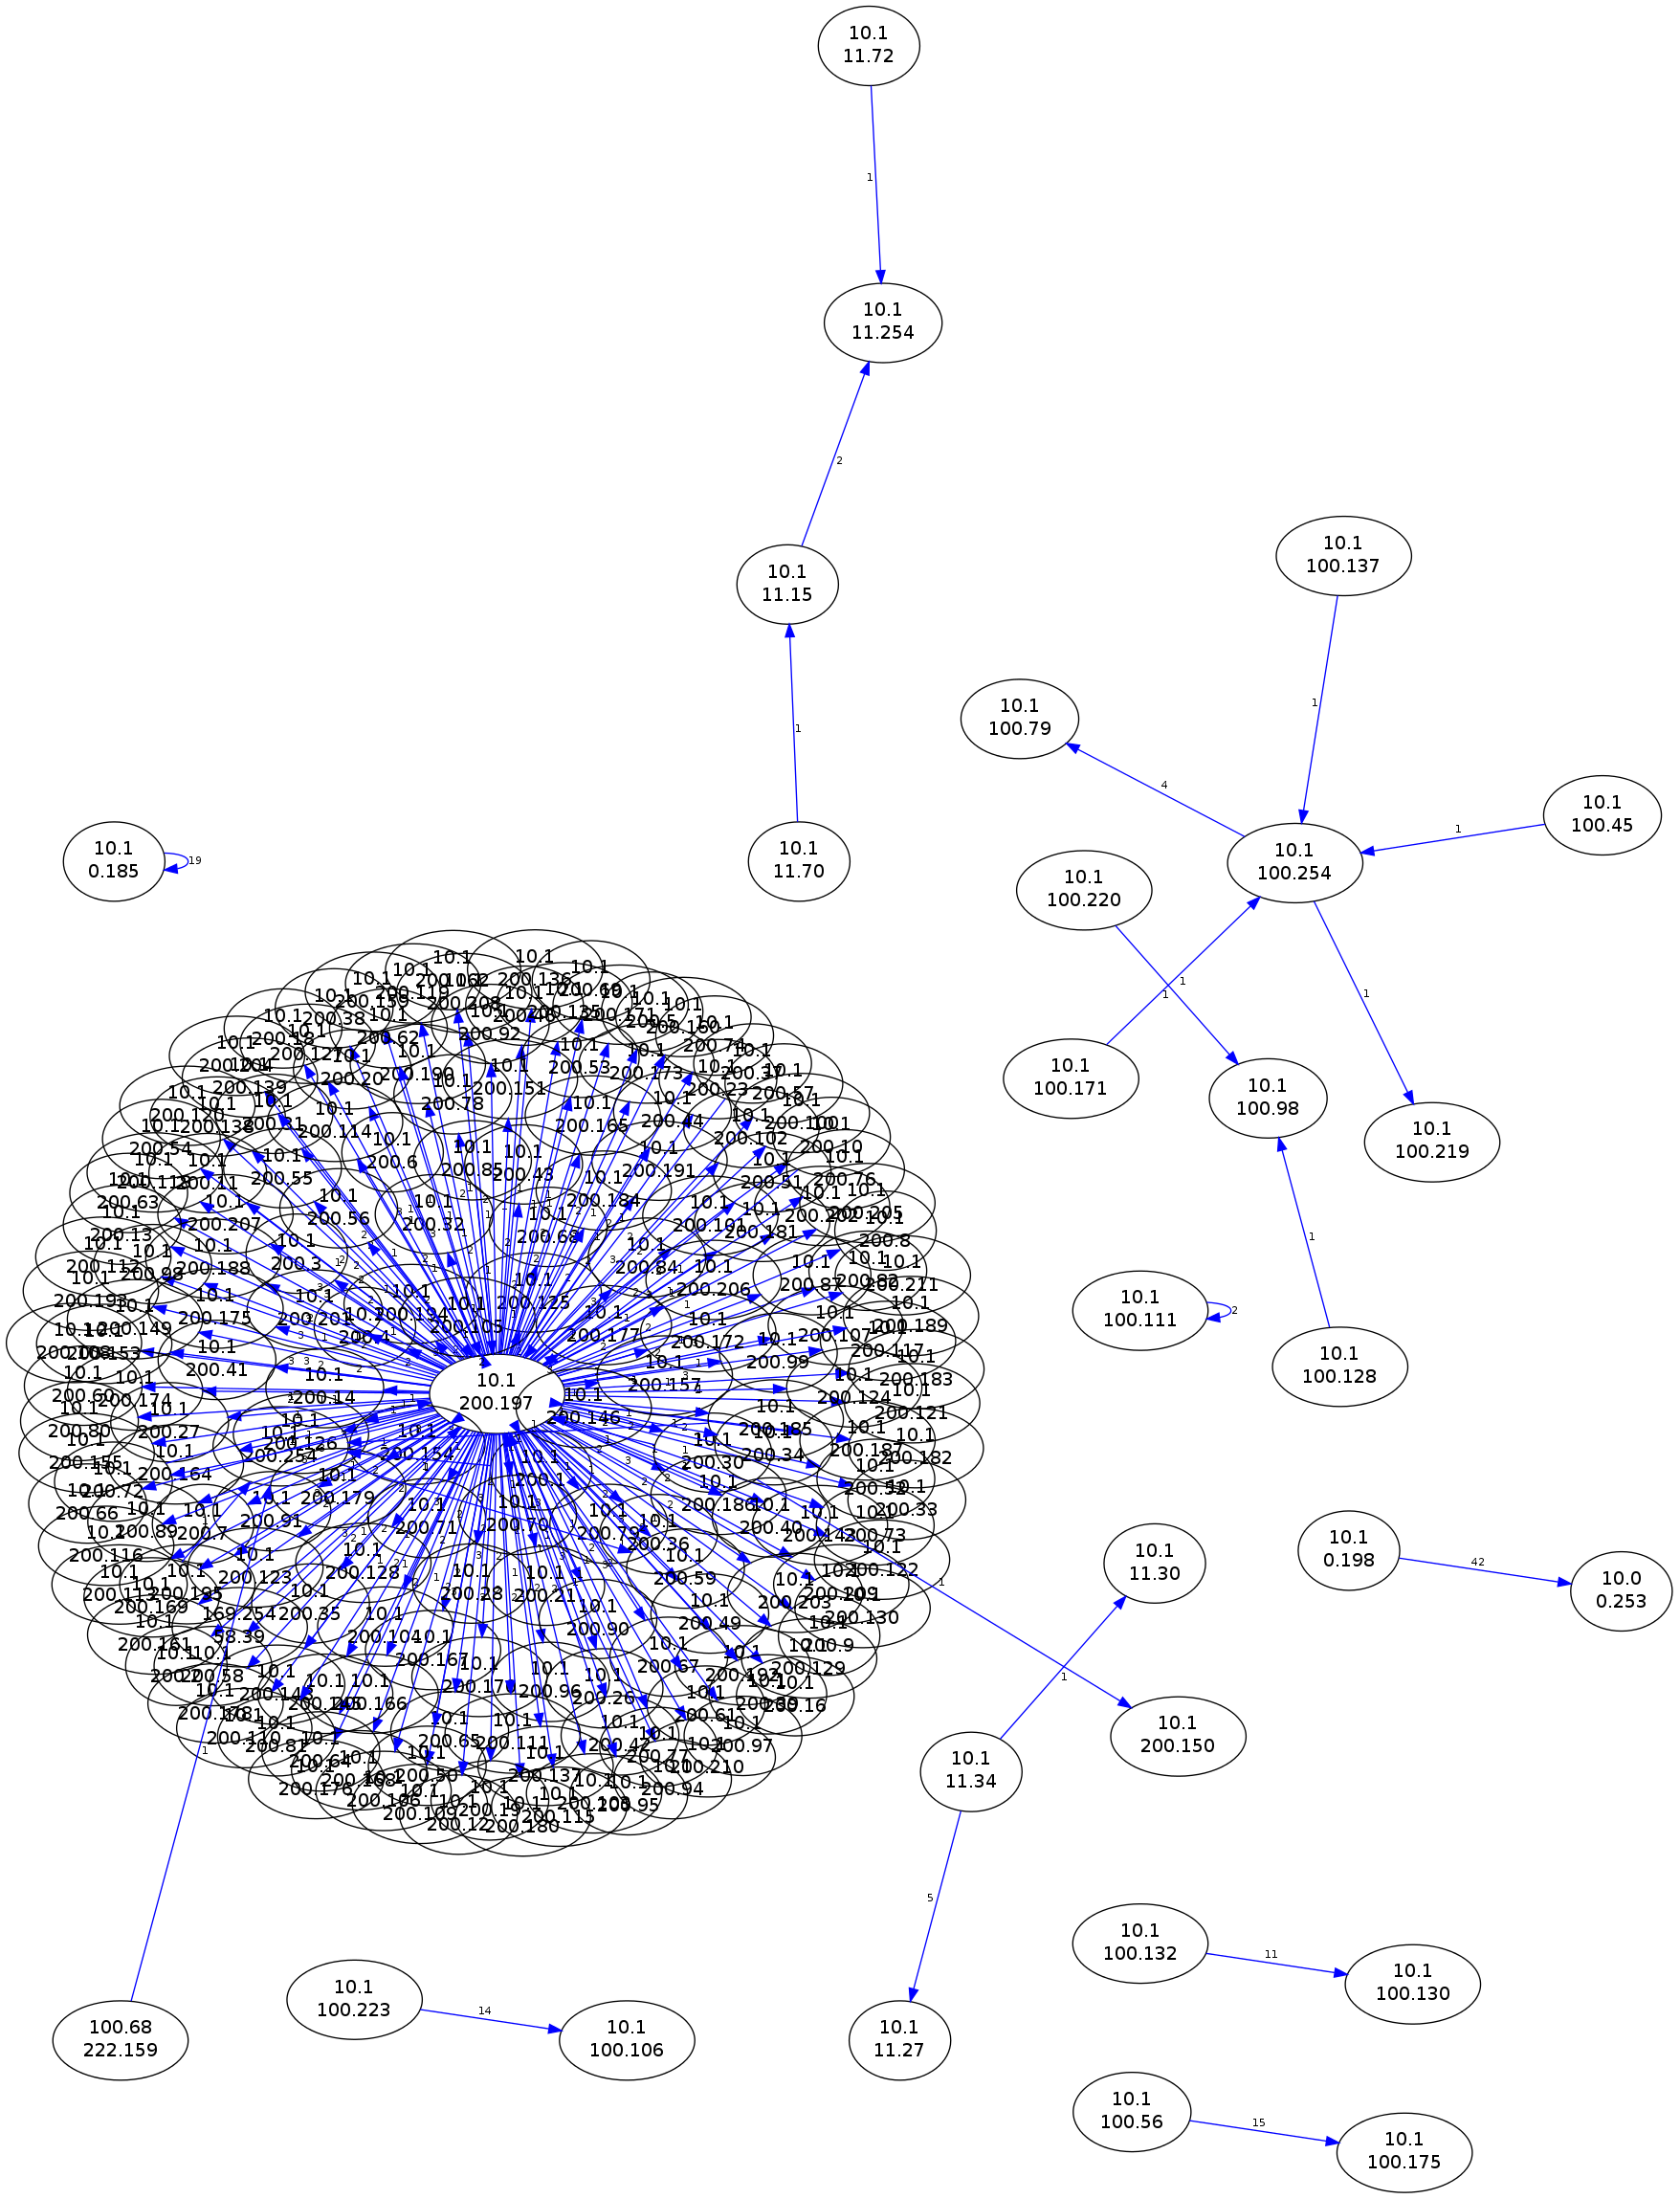
\includegraphics[width=0.6\linewidth]{../imgs/red-entrepiso-dc_red.png}
    \caption{Grafo mostrando la topología de la red \emph{Entrepiso-DC}.}
    \label{fig:entrepiso-dc-grafo}
  \end{center}
\end{figure}

\subsubsection{Fuente: $S_{dst}$}

\begin{figure}[H]\centering
    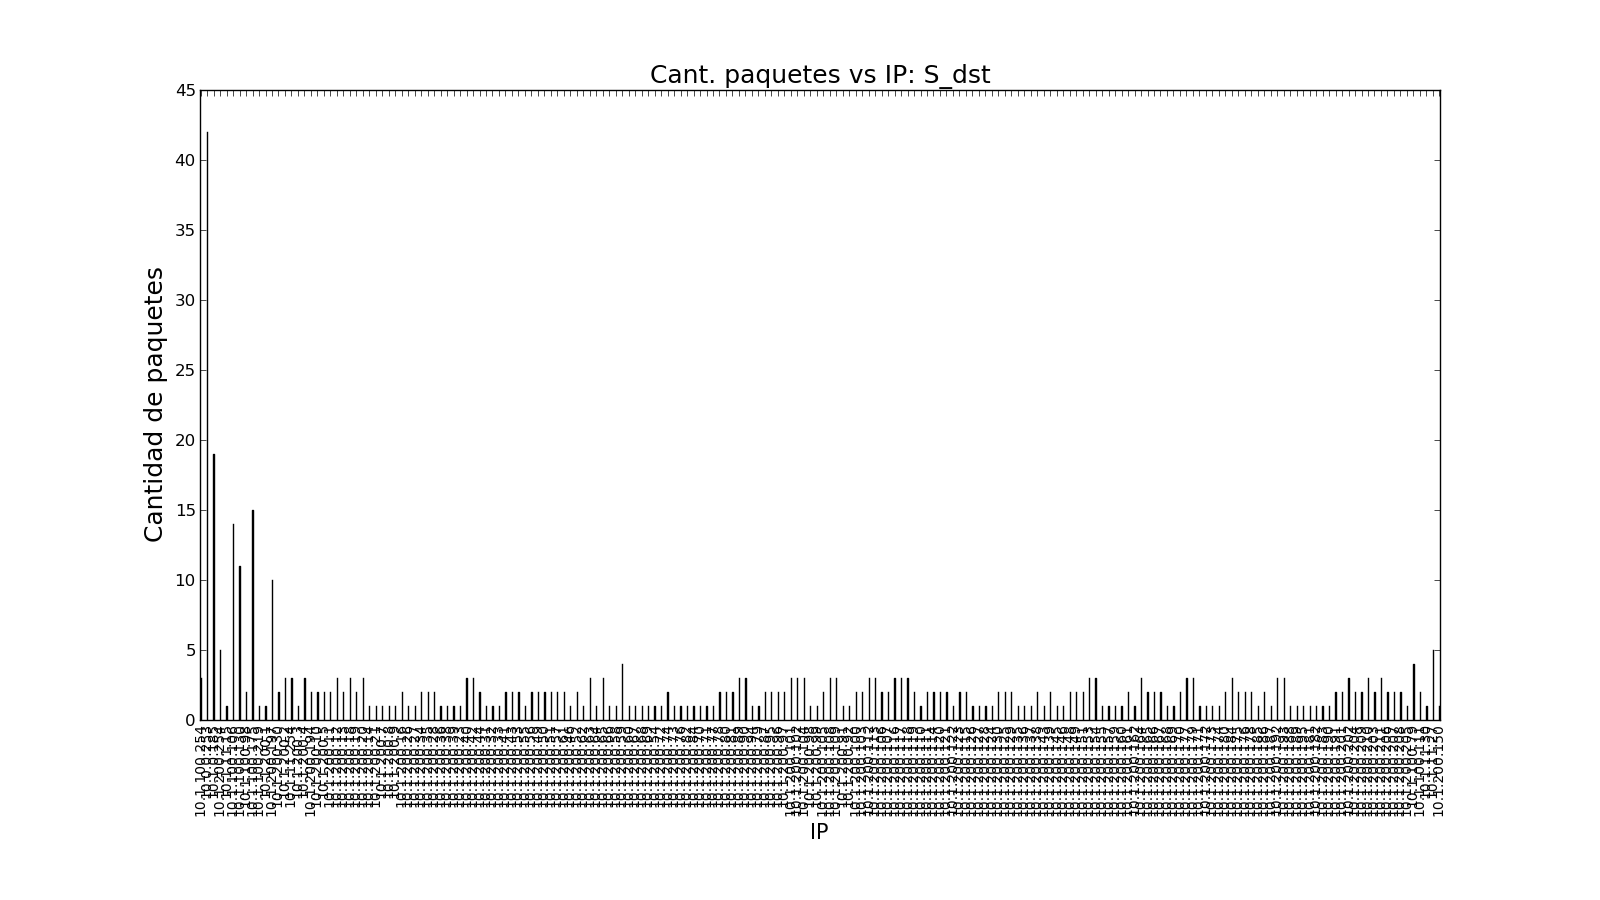
\includegraphics[width=\linewidth]{../imgs/red-entrepiso-dc_S_dst_hist.png}
    \caption{Histograma de $S_{dst}$}\label{fig:entrepiso-dc-dst-hist}
\end{figure}

\begin{figure}[H]\centering
    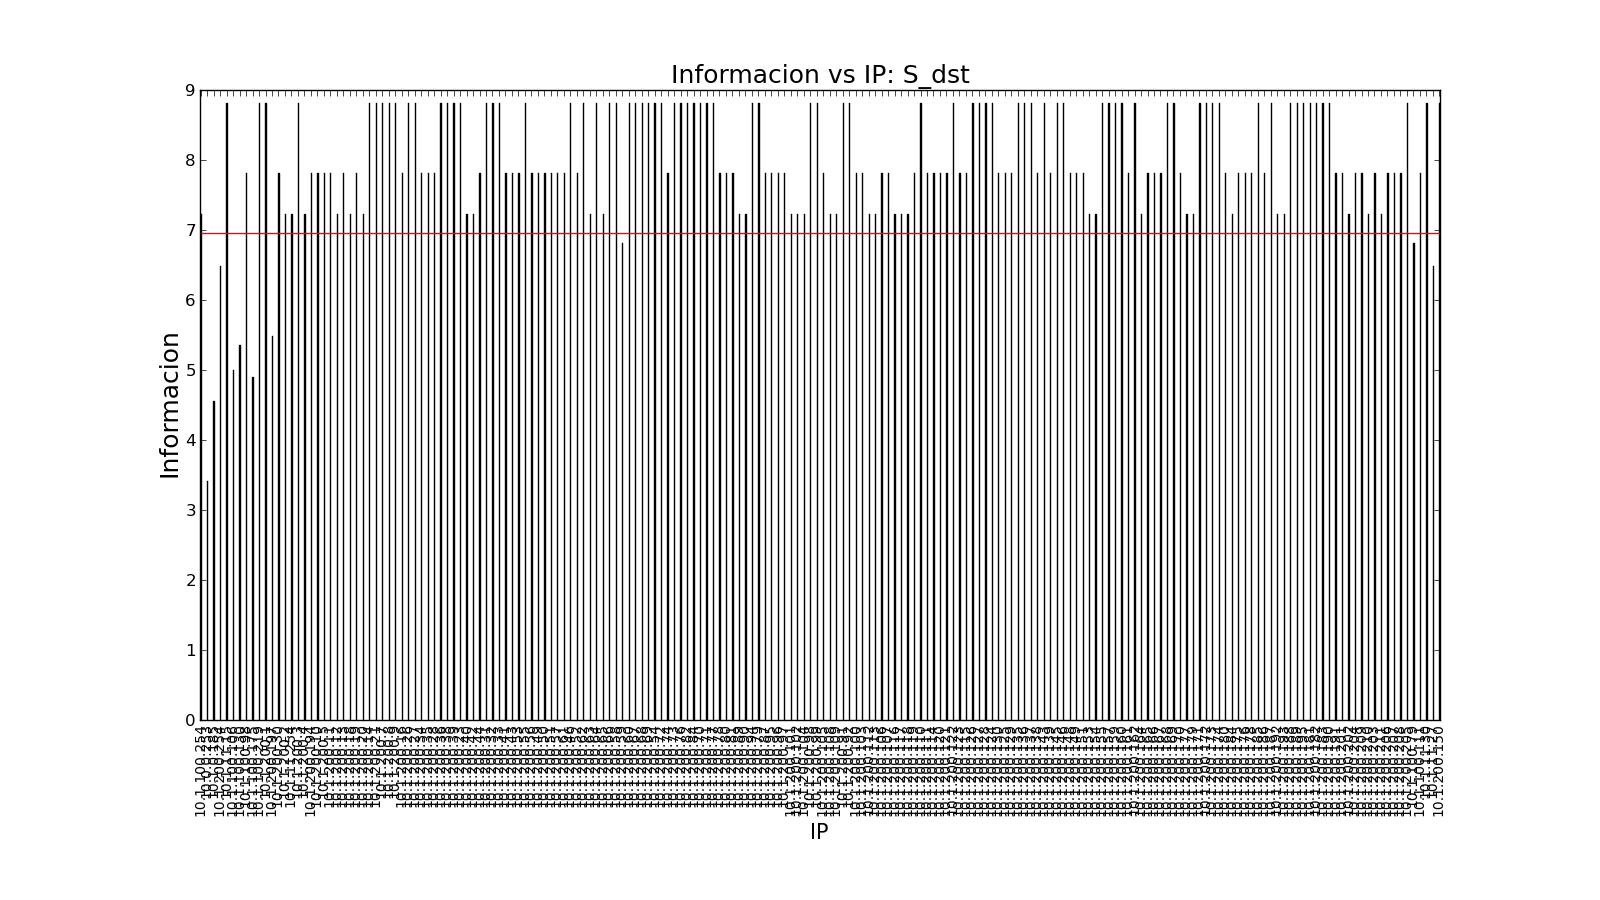
\includegraphics[width=\linewidth]{../imgs/red-entrepiso-dc_S_dst_info.png}
    \caption{Informacion de $S_{dst}$}\label{fig:entrepiso-dc-dst-info}
\end{figure}

$\bullet$ Entropía de la fuente: 6.95 sobre un máximo posible de 7.58

En las figuras \ref{fig:entrepiso-dc-dst-hist} y \ref{fig:entrepiso-dc-dst-info} se presentan los gráficos tipo histograma e información para la fuente $S_{dst}$. En este caso, hay múltiples nodos con una frecuencia mucho mayor que la media, siendo distinguidos aproximadamente 10 nodos según el criterio de la sección \ref{subsec:modelos-fuente-informacion}.

\subsubsection{Fuente: $S_{src}$}

\begin{figure}[H]\centering
    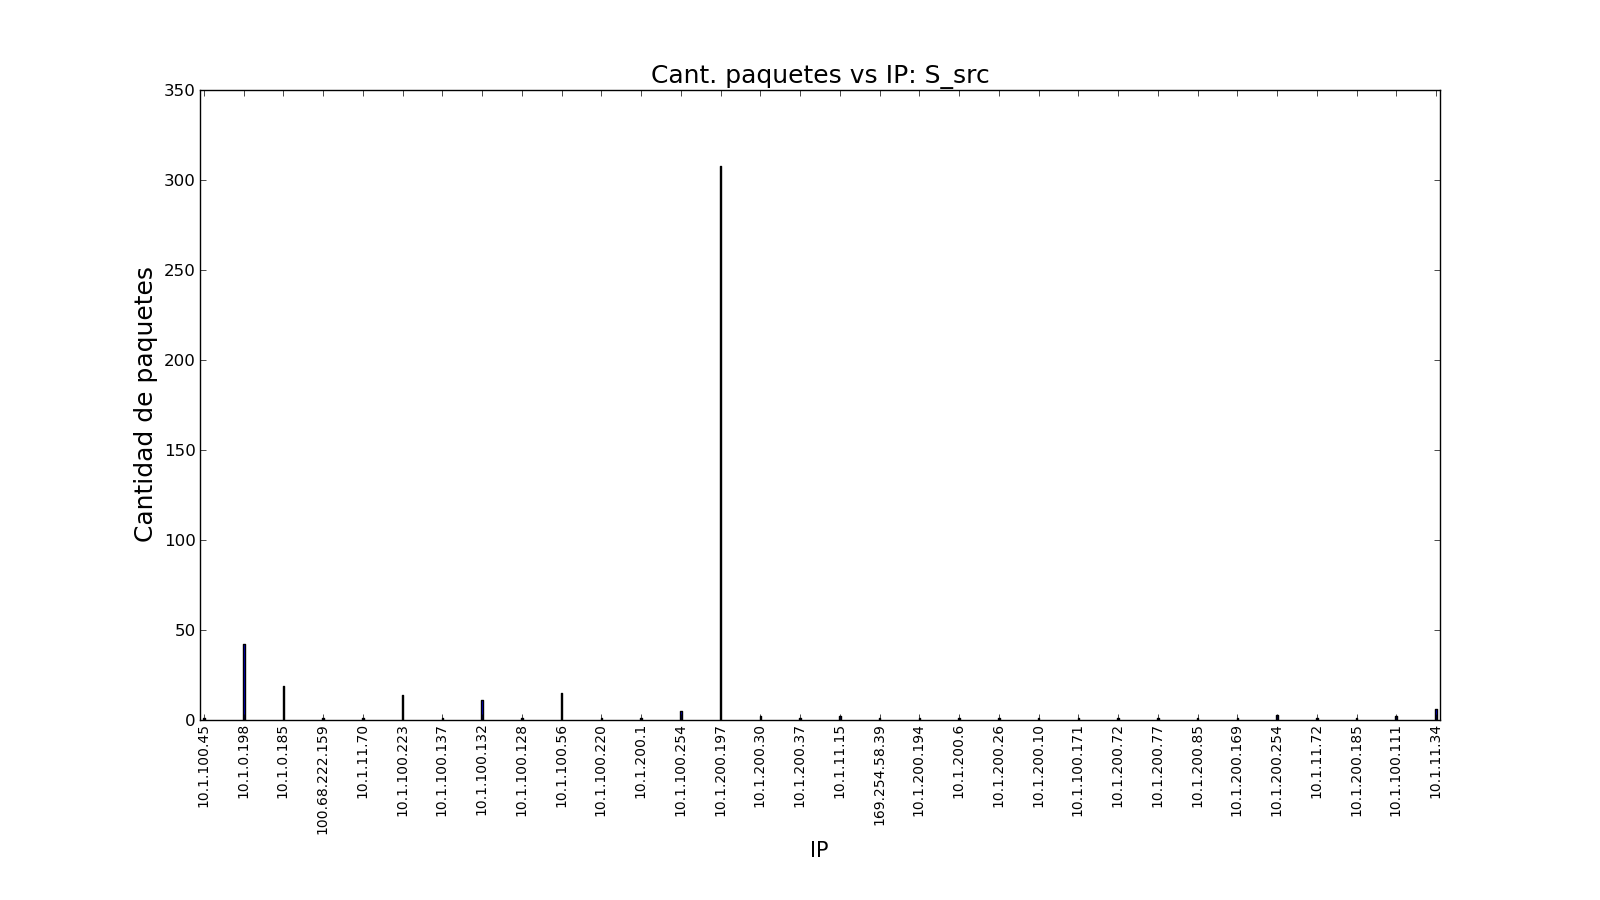
\includegraphics[width=\linewidth]{../imgs/red-entrepiso-dc_S_src_hist.png}
    \caption{Histograma de $S_{src}$}\label{fig:entrepiso-dc-src-hist}
\end{figure}

\begin{figure}[H]\centering
    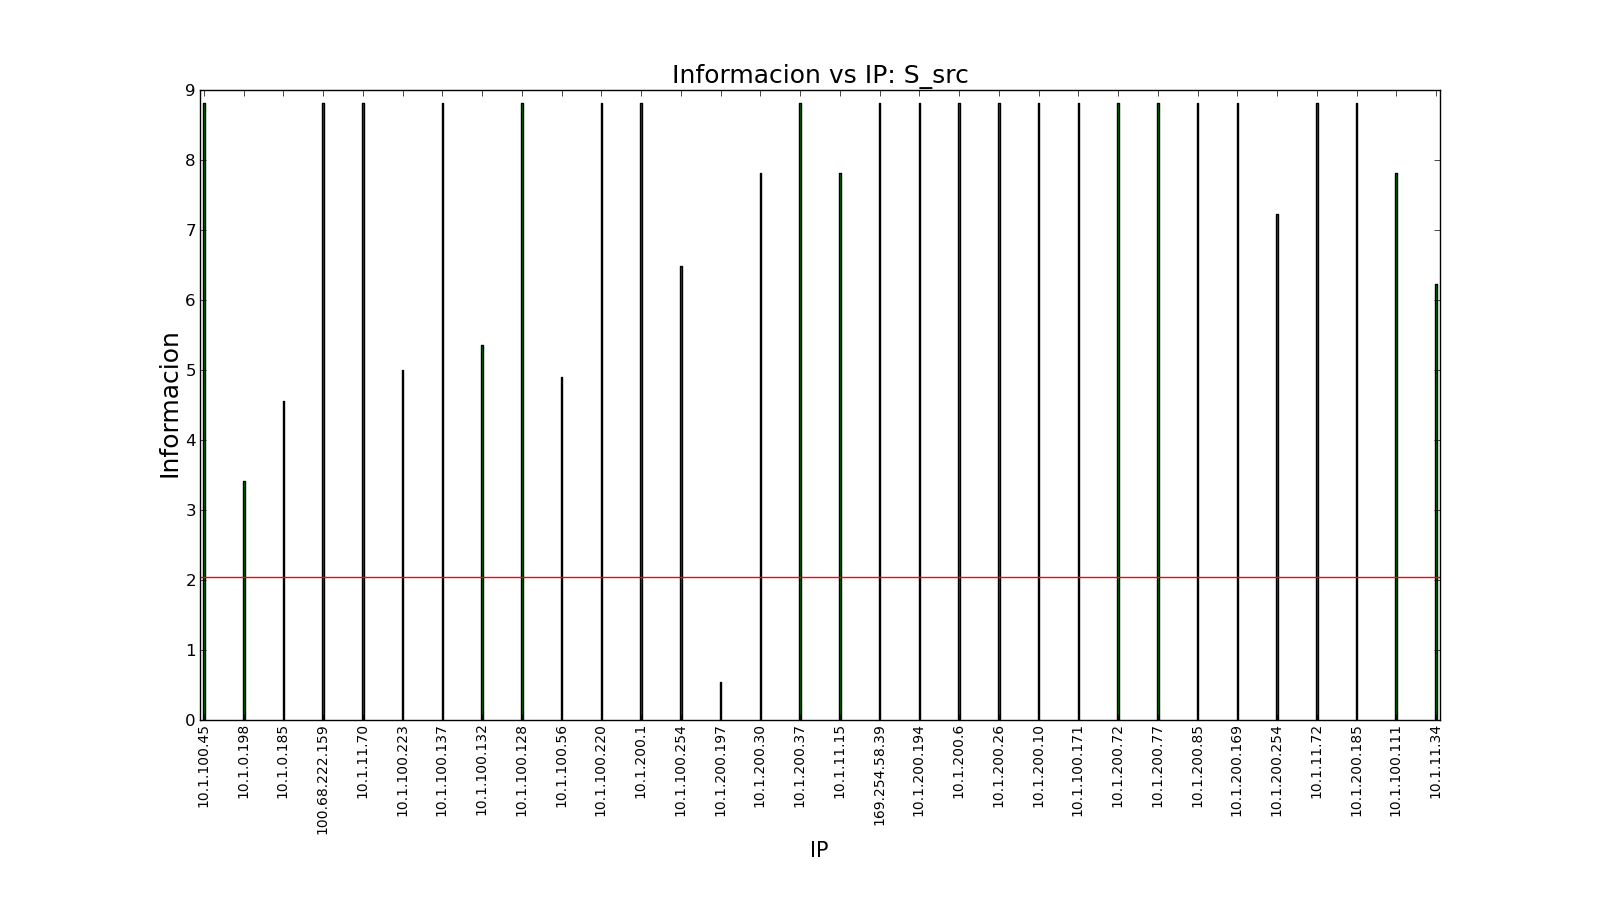
\includegraphics[width=\linewidth]{../imgs/red-entrepiso-dc_S_src_info.png}
    \caption{Informacion de $S_{src}$}\label{fig:entrepiso-dc-src-info}
\end{figure}

$\bullet$ Entropía de la fuente: 2.03 sobre un máximo posible de 5.00

En las figuras \ref{fig:entrepiso-dc-src-hist} y \ref{fig:entrepiso-dc-src-info} se presentan los gráficos tipo histograma e información para la fuente $S_{src}$. A diferencia de la fuente $S_{dst}$, en este caso hay un único nodo distinguido, el de IP \emph{10.1.200.197}.

\subsubsection{Discusión}

En el caso de esta red, la entropía de la fuente $S_{dst}$ es mucho más alta en términos relativos (92\% de la máxima posible) que la de la fuente $S_{src}$ (41\%). Esto es previsible dados los gráficos de información, dado que $S_{src}$ tiene una estructura más jerarquizada respecto al nodo distinguido; complementándose con lo que se observa en el gráfico del grafo.
Enfocando el análisis el cluster que aglomera la mayor cantidad de nodos, la IP \emph{10.1.200.197} es la que envía y recibe mayor cantidad de paquetes, y por lo tanto pareciera tratarse del gateway.

Suponemos que son pequeños grupos de terminales que se comunican entre sí, pero no con el conjunto general (que suponemos que lleva a Internet). Una posibilidad es que sean máquinas de oficina que accedan entre si, o a una terminal que da un servicio (ej. impresora).
  
\section{Discusión General}
En esta sección vamos a discutir acerca de las distintas entropías de las distintas fuentes de las redes observadas.

\begin{center}
\textbf{Red Hogareña}

\begin{tabular}{|c|c|c|c|}
\hline
Fuente&Entropía H(S)&Entropía Máxima&Proporción\\
\hline
$S_{dst}$&1.27&1.58&0.80\\
$S_{src}$&1.23&2.0&0.62\\ 
\hline
\end{tabular}
\end{center}

\begin{center}
\textbf{Red Alto Palermo}

\begin{tabular}{|c|c|c|c|}
\hline
Fuente&Entropía H(S)&Entropía Máxima&Proporción\\
\hline
$S_{dst}$&4.66&6.54&0.71\\
$S_{src}$&4.96&6.73&0.74\\ 
\hline
\end{tabular}
\end{center}

\begin{center}
\textbf{Red Honeywell}

\begin{tabular}{|c|c|c|c|}
\hline
Fuente&Entropía H(S)&Entropía Máxima&Proporción\\
\hline
$S_{dst}$&3.17&4.39&0.72\\
$S_{src}$&2.05&3.32&0.62\\ 
\hline
\end{tabular}
\end{center}

\begin{center}
\textbf{Red Entrepiso-DC}
 
  \begin{tabular}{|c|c|c|c|}
  \hline
  Fuente&Entropía H(S)&Entropía Máxima&Proporción\\
  \hline
  $S_{dst}$&6.96&7.58&0.92\\
  $S_{src}$&2.04&5.00&0.41\\ 
  \hline
  \end{tabular}
\end{center}

Como podemos observar, los valores de la proporción entre la entropía y la entropía máxima de las fuentes rondan los 0.60 y 0.80 salvo en la Red Entrepiso. En dicha red, los valores son mas dispares. 

En la Red Hogareña, podemos ver que en la fuente $S_{src}$ la proporción es más baja lo cual implica que hay menos incertidumbre en dicha fuente. Esto significa que la cantidad de paquetes ARP \emph{who-has} enviados no esta uniformemente distribuida entre las distintas IPs. Por otro lado, en $S_{dst}$ la proporción es más alta lo cual implica que hay más incertidumbre en esa fuente. Esto quiere decir que los paquetes recibidos tienen una distribución más uniforme que en la fuente $S_{src}$.

Esto se repite de manera análoga en la Red Honeywell. Sin embargo, cabe aclarar que la entropía máxima en la Red Honeywell es mayor a la entropía máxima de la Red Hogareña en ambas fuentes. Esto significa que hay más IPs involucradas en los paquetes de las fuentes.

En la Red Alto Palermo, ambas las proporciones de ambas fuentes son similares. Esto significa que su distribución tiene uniformidad parecida.

Finalmente, en la Red Entrepiso la proporciones son las más distantes. La distribución de la fuente $S_{dst}$ es la más uniforme de todas, lo cual es reflejado en su alta proporción (0.92). Por otro lado, la proporción de $S_{src}$ es la más baja de todas. Esto significa que esta fuente es la que tiene menos incertidumbre de todas.

La entropía máxima de las distintas fuentes $S_{dst}$ tiene un máximo de 7.58 en su homónima de la Red Entrepiso. Por otro lado, la entropía máxima de las fuentes $S_{src}$ tiene su máximo en la Red Alto Palermo, con un valor de 6.73.

\newpage

\section{Conclusiones}
Como conclusión, queremos recalcar que por lo general los routers son nodos distinguidos en las LANs a las que pertenecen, ya que el router funciona como \emph{gateway}. Esto se mantiene, ya sea una red pública o privada.

Como pudimos ver en los experimentos, creemos que es importante saber que un nodo distinguido no siempre es un router. En el caso de Red Entrepiso, creemos que el servidor local era un nodo distinguido.

Para finalizar, en este trabajo práctico pudimos ver que no necesariamente un nodo distinguido es distinguido tanto en $S_{src}$ como en $S_{dst}$.



\end{document}	